\chapter{Introduction}
\enlargethispage{3\baselineskip}

\begin{keypointstwomargins}{Introduction}{-2cm}{-1cm}

        \textbf{Key points -- Crowdsourcing in todays spectrum}
        \begin{enumerate}[leftmargin=*]

        \item In the deep learning era we create bigger and bigger datasets, using labels that are not always correct. The prediction quality of a model follows the input data quality. Can we mitigate the impact of the noise induced by the data collection process?

        \item Handling crowdsourcing data comes with two main strategies: either aggregate the collected labels and then use supervised learning from them. Or directly integrate a model that mitigates the crowd noise inside the neural network's architecture. However, most models deal with worker quality, few consider data difficulty.

        \item Research has been made into trying to better learn the prediction uncertainty for a neural network by inducing noise in the label distribution. Using crowdsourced data, we have a direct access to the human uncertainty. However, this data is rarely openly available, making crowdsourcing experiments hard to reproduce and compare.

        \end{enumerate}

        \textbf{Contributions -- Crowdsourcing: from the worker to the task and back}
        \begin{enumerate}[leftmargin=*,start=4]
        \item Following research on labeling noise in supervised datasets, we adapt the AUM into the WAUM to help detect highly ambiguous images in crowdsourced datasets.

        \item We emphasize the need for reproducible results and shared algorithms with the creation of a crowdsourcing library: \texttt{peerannot}. This lets us easily compare scoring metrics for workers depending on the strategy used and their use case.

        \item We discuss the need for more openly available crowdsourced datasets and the limitations of currently accessible ones.
        \end{enumerate}

\end{keypointstwomargins}

\section{Crowdsourcing in computer vision}

Following the deep learning revolution, models with millions if not billions of parameters to optimize are trained nowadays. And to do so, we need to increase the size of our training datasets.
The issue is, that in a training set in supervised classification (and we will mainly consider image classification for the rest of this work), the images need to come with a label to train from.
While research has been conducted on inferring this label from the data itself, in the classical supervised learning datasets these labels have been collected and shared at some point during the creation of the dataset.

\begin{figure}[ht]
    \centering
    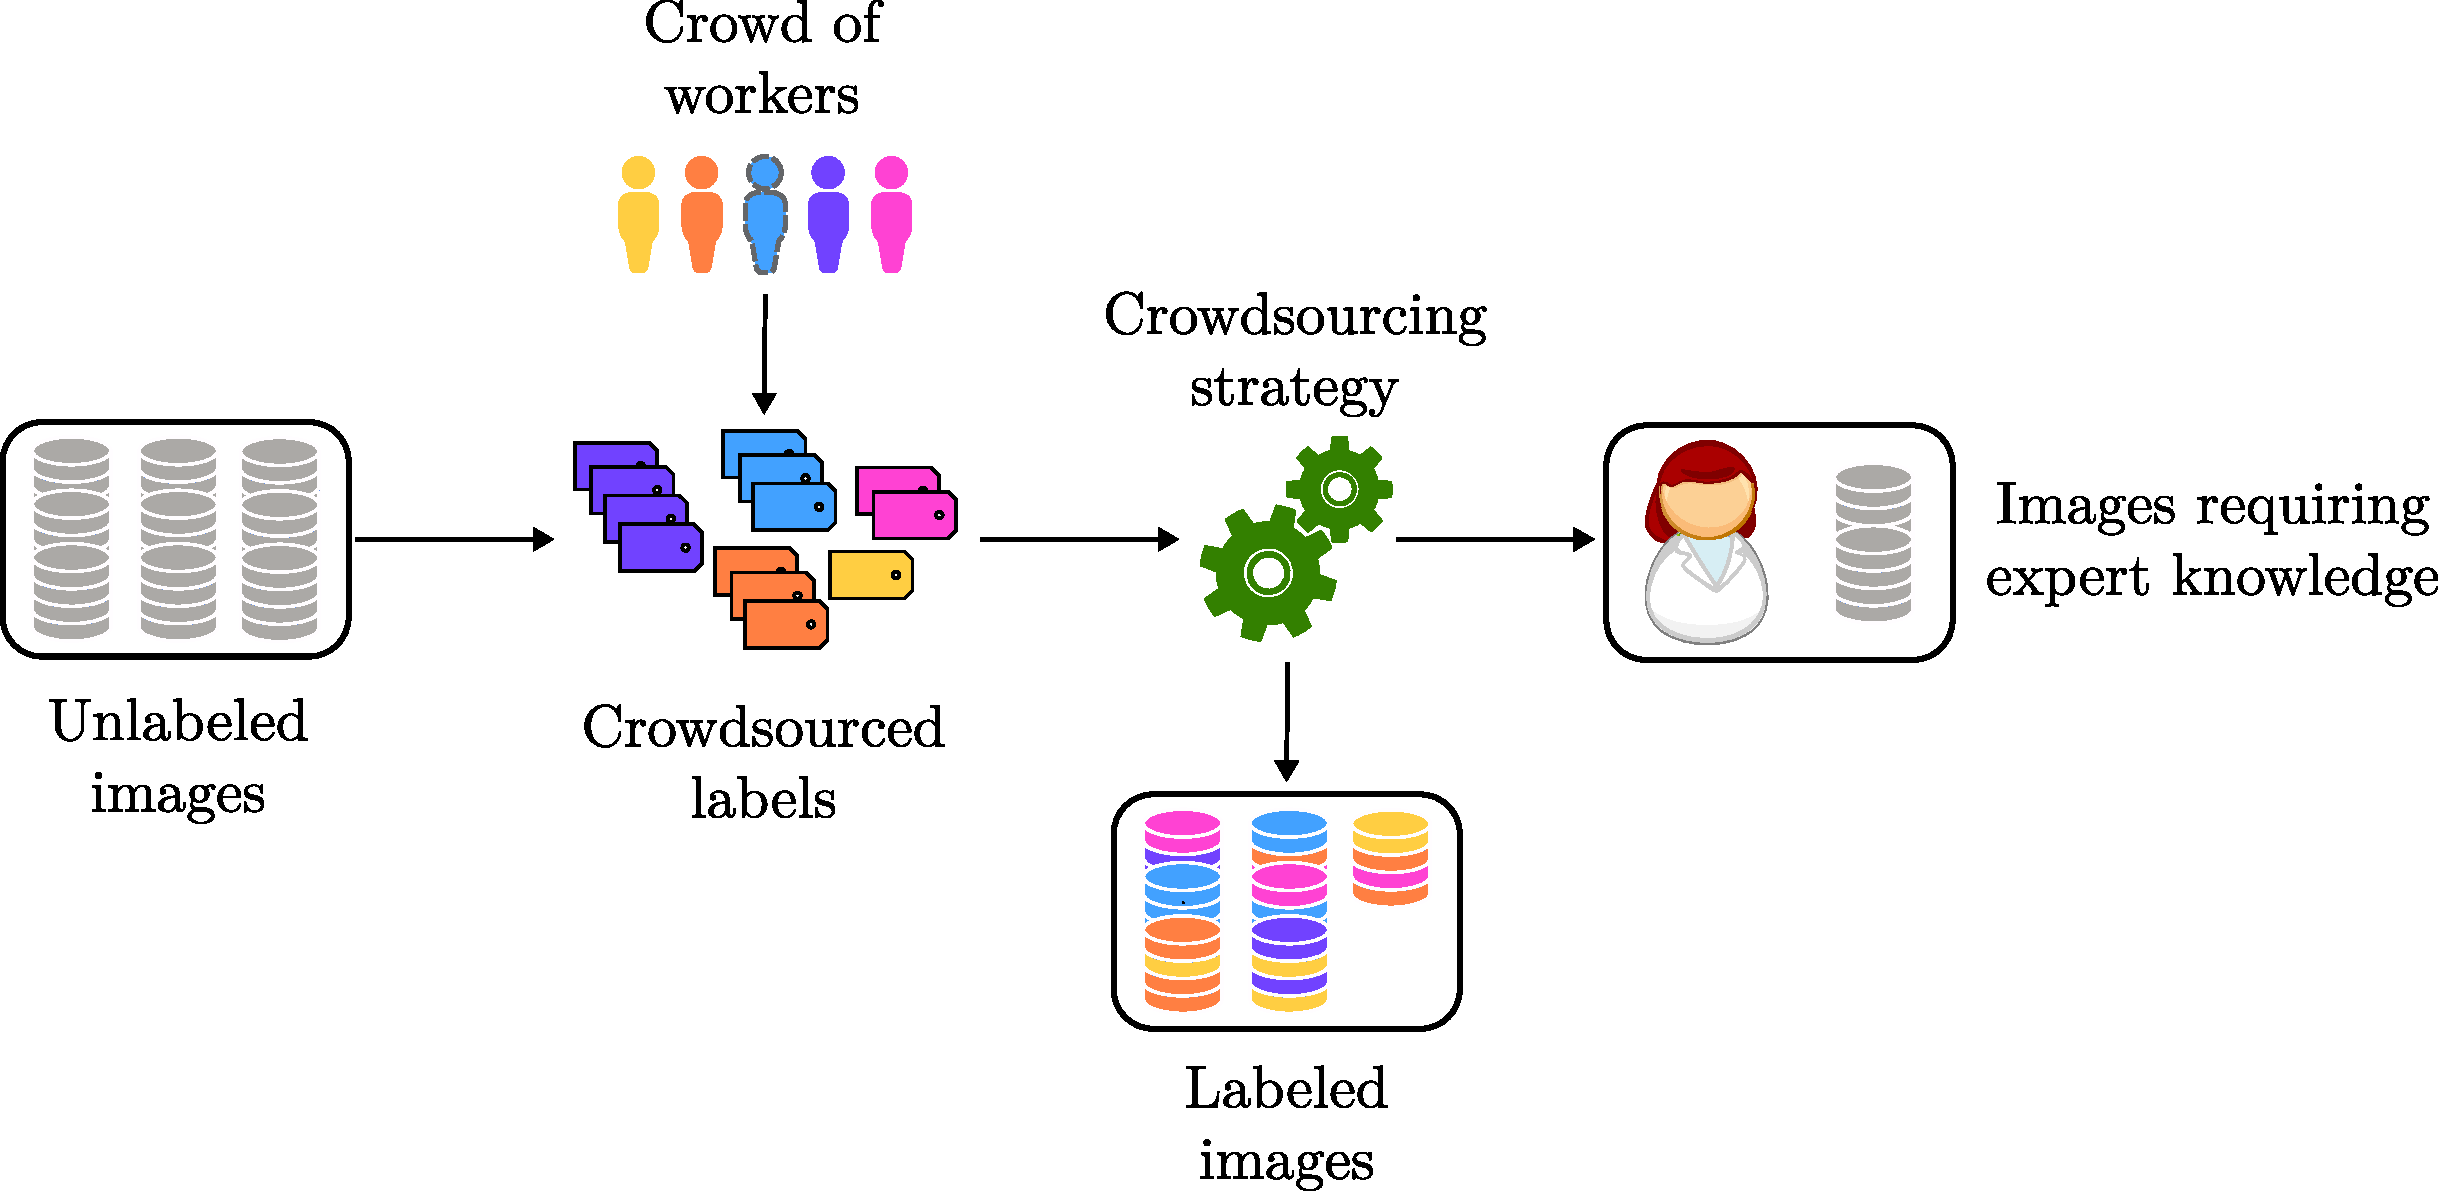
\includegraphics[width=.8\textwidth]{chapters/images/expert_knowledge.pdf}
    \caption{Crowdsourcing can be used to create datasets, but also relieves the tension experts receive in evaluating new data. By using a crowd of workers, many tasks can be labeled without needing expert evaluation.}
    \label{fig:expert_knowledge}
\end{figure}

The task of collecting data to create a dataset for image classification has been more and more linked with web-scrapping \citep{rhodes2015vaping}.
However, it has been shown numerous times that labeling mistakes do happen with this data collection strategy \citep{northcutt_pervasive_2021,vasudevan2022does}.
In other fields of research, as healthcare providers, images might not come from the web but are collected between multiple locations -- like hospital scanners.
When trying to classify a scanner as \emph{"presence or absence of tumors"}, it is often a field expert that provides the label.
However such healthcare providers can't label thousands of images.
In this case, the power of the crowd can be used to label the scans and provide some level of uncertainty.
This is then to the data scientist area, in collaboration with experts, to determine which workers were useful in the experiment, and which were not, and then only ask experts to label the most ambiguous scans -- which would represent only a small fraction of the original dataset (as illustrated in \Cref{fig:expert_knowledge}).

\subsection{Crowdsourcing is all over}

This collaboration between citizens and scientists is not technically niche, only quite often it goes unnoticed.
Using crowdsourcing to collect data has been used in medical science, video recommendation systems, and so many other fields of research and development.
We wish to show a -- non-exhaustive and not ordered -- list of such projects relying on human interactions to collect data, not just for image classification:
\begin{itemize}
    \item Pl@ntNet: plant species recognition application \citep{plantet},
    \item Eyewire: a game to map retina's neurons \citep{tinati2017investigation},
    \item Tournesol: public interest YouTube video recommendation system \citep{hoang2021tournesol},
    \item ChatGPT: evaluate and correct prompt quality \citep{openai2023gpt4},
    % \item Waze: traffic conditions, presence of dangers on the road\footnote{\url{https://assets.brandfolder.com/pbtsls-1nska8-dxoeew/original/Waze_Company.pdf?_ga=2.186820589.494513673.1542075282-1186534970.1542075282}},
    \item Duolingo: traduction corrections and improvements\footnote{\url{https://www.theguardian.com/education/2014/aug/27/luis-von-ahn-ceo-duolingo-interview}},
    \item RTR: photovoltaic panels segmentation in images \citep{kasmi2023crowdsourced},
    \item Twitter/$\mathbb{X}$ via Birdwatch: identify misleading information \citep{wojcik2022birdwatch},
    \item Spotify\footnote{\url{https://community.spotify.com/t5/Content-Questions/Shutting-down-Line-In/td-p/4557664}}, TripAdvisor\footnote{\url{https://www.kingigilbert.com/crowdsourcing-tripadvisor/}}, SNCF\footnote{\url{https://www.usine-digitale.fr/article/tranquilien-quand-open-data-et-crowdsourcing-profitent-aux-voyageurs-franciliens.N200017}},\dots
\end{itemize}

With this list, we showcase the large domains of applications of keeping humans -- and citizens -- in the loop, and thus the need for more research on crowdsourcing settings, strategies and implications.
In this thesis, we mainly focus on the image classification setting.

\subsection{The Pl@ntNet project}
Created by Alexis Joly and Pierre Bonnet, Pl@ntNet \citep{plantet} is the meeting of two communities -- botanists and computer science -- to identify plant species from photos taken on the spot.
The project's birth began in 2008, released its first web application in 2011, mobile application in 2013 and received in 2020 the price \emph{Prix de l’innovation Inria – Académie des sciences – Dassault Systèmes}.
\begin{figure}[tbh]
    \centering
    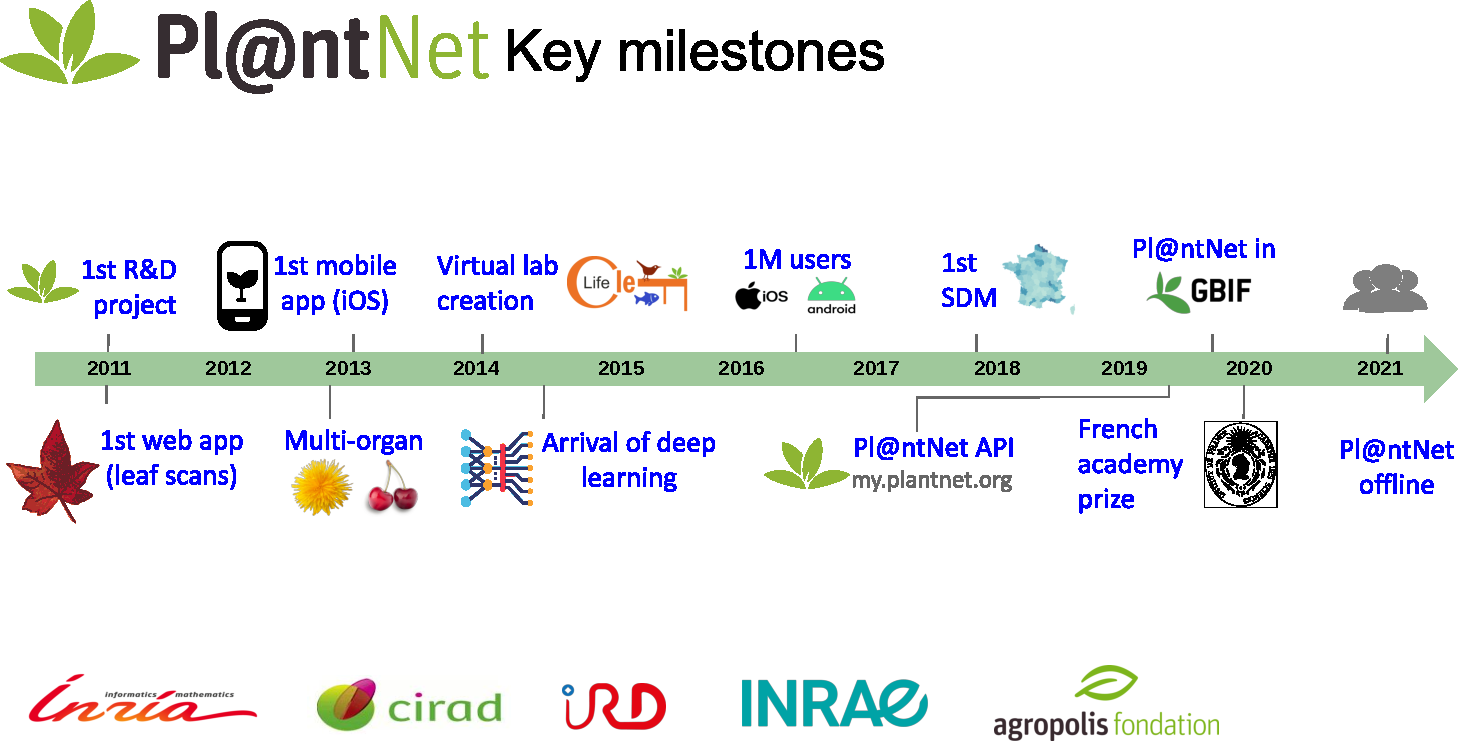
\includegraphics[width=.8\textwidth, clip, trim={0cm 0cm 0cm 2.5cm}]{chapters/images/Pl@ntNet-overview-Janv-2022.pdf}
    \caption{Timeline of the Pl@ntNet project}
    \label{fig:timeline-plantnet}
\end{figure}

The Pl@ntNet system can be interpreted as follows. A user records an observation (an image or group of images from the same plant) and sends a query for identification.
The current version of Pl@ntNet's computer vision model (referred to as Pl@ntNet's AI model and detailed in \Cref{chap:plantnet}) makes a prediction and outputs the most probable species.
The user can then agree with the AI model, or input another species.
With the predicted probabilities, similar observations with indicated species are shown to the user to help them make their decision.
The observation is then shared (based on the user's consent) with the community and can be voted on by other users.

\begin{figure}[htb]
    \centering
    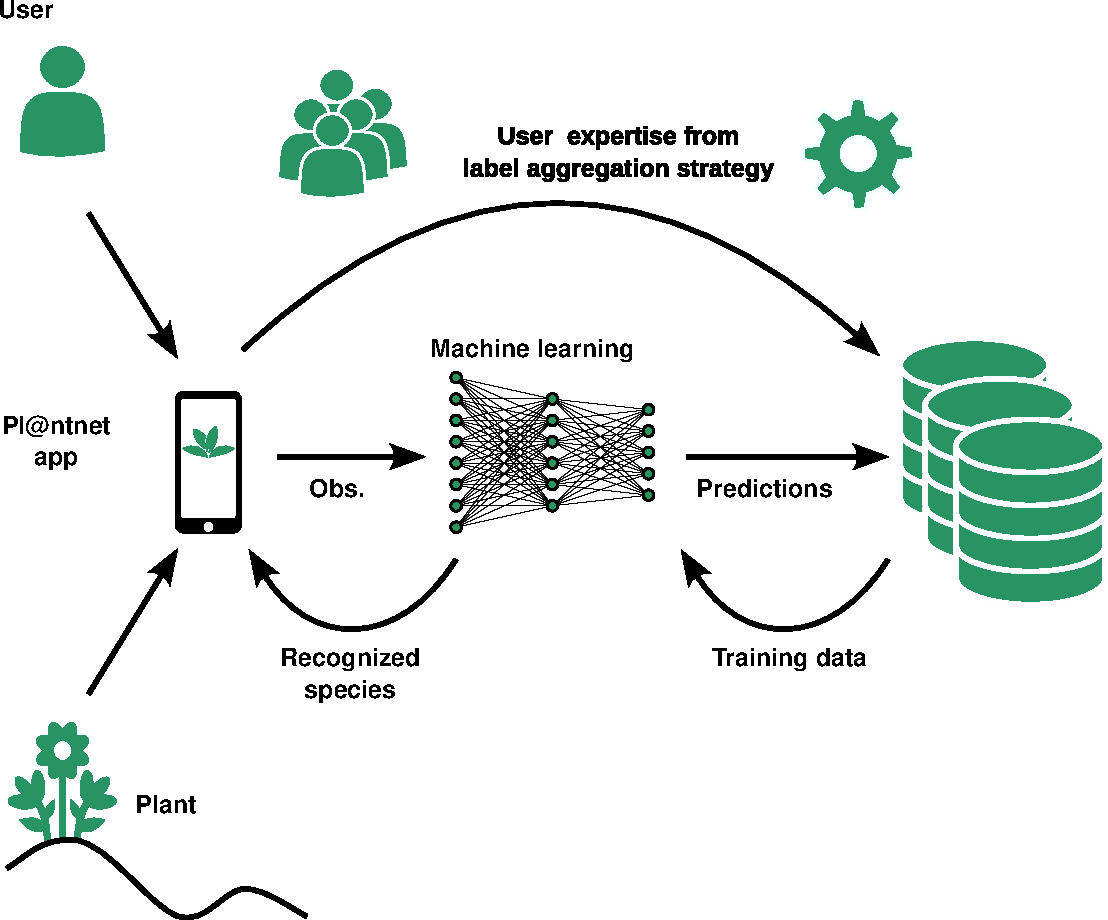
\includegraphics[width=.65\textwidth]{chapters/images/plantnet_schema_global_green.pdf}
    \caption{Pl@ntNet pipeline from the observation taken in the field to the active training of the computer vision model.}
    \label{fig:pipeline-plantnet}
\end{figure}

Once the observation is registered, it can be revised at any time by other users.
Currently, Pl@ntNet records over $50$K species, $6$M registered users and $21$M observations spread across $77$ floras.
Over a billion image queries have been made, and the application has been downloaded over $10$M times on Google AppStore.
In total, more than $22$M votes have been cast internationally.
Each publicly shared observation presents, as in \Cref{fig:interface-plantnet} with an associated author, the current votes and the state of the current species determination.
On the platform, users can vote for a malformed label, if the picture is about a leaf, a flower, a fruit, the bark, the habit or other. In this thesis, we only consider the species determination, not the other votes.

\begin{figure}[H]
    \centering
    \begin{minipage}{.55\linewidth}
        \centering
        \subfloat[Identification webpage. The observation is composed of two pictures, one of the organ (left) and the other of the flower (right).]{\label{fig:interface}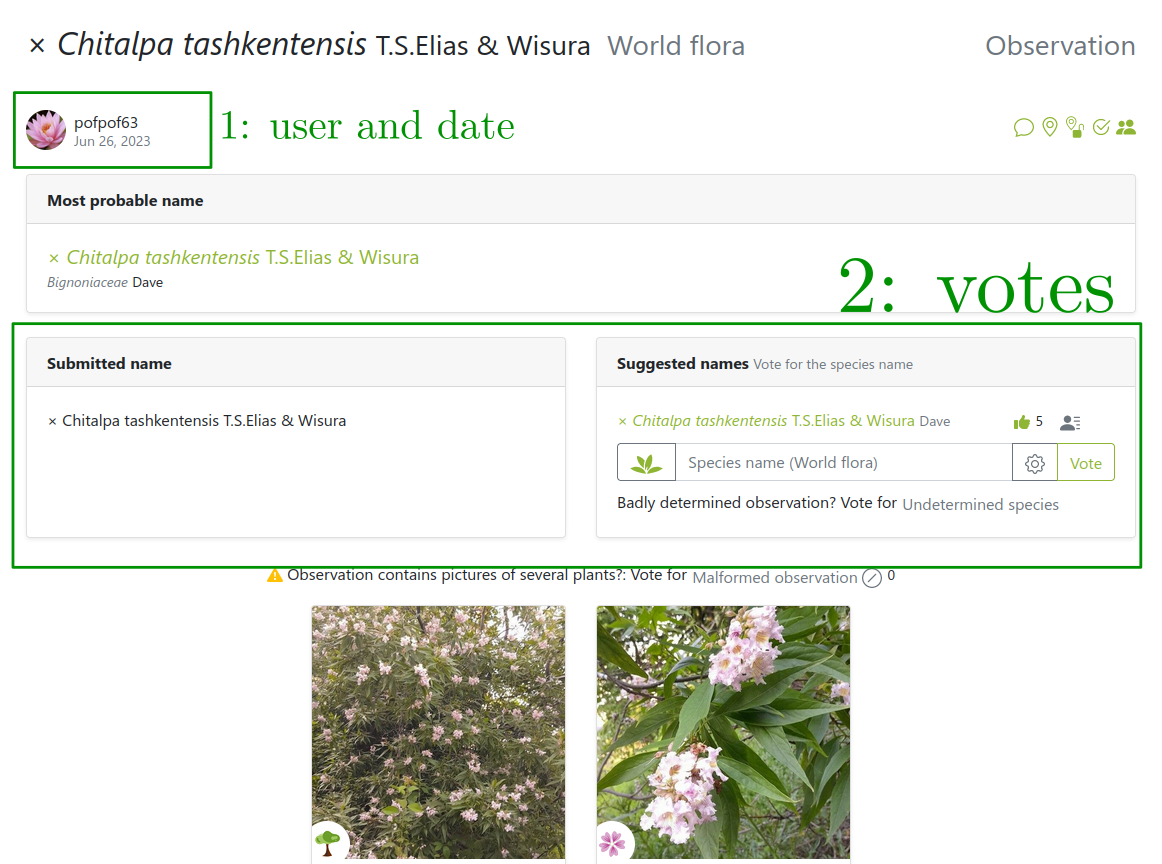
\includegraphics[width=\textwidth]{chapters/images/plantnet_online.png}}
        \end{minipage}%
        \hfill
        \begin{minipage}{.4\linewidth}
        \centering
        \subfloat[User vision of current model predictions. Examples for each species are proposed for visual comparison.]{\label{fig:interface-ai}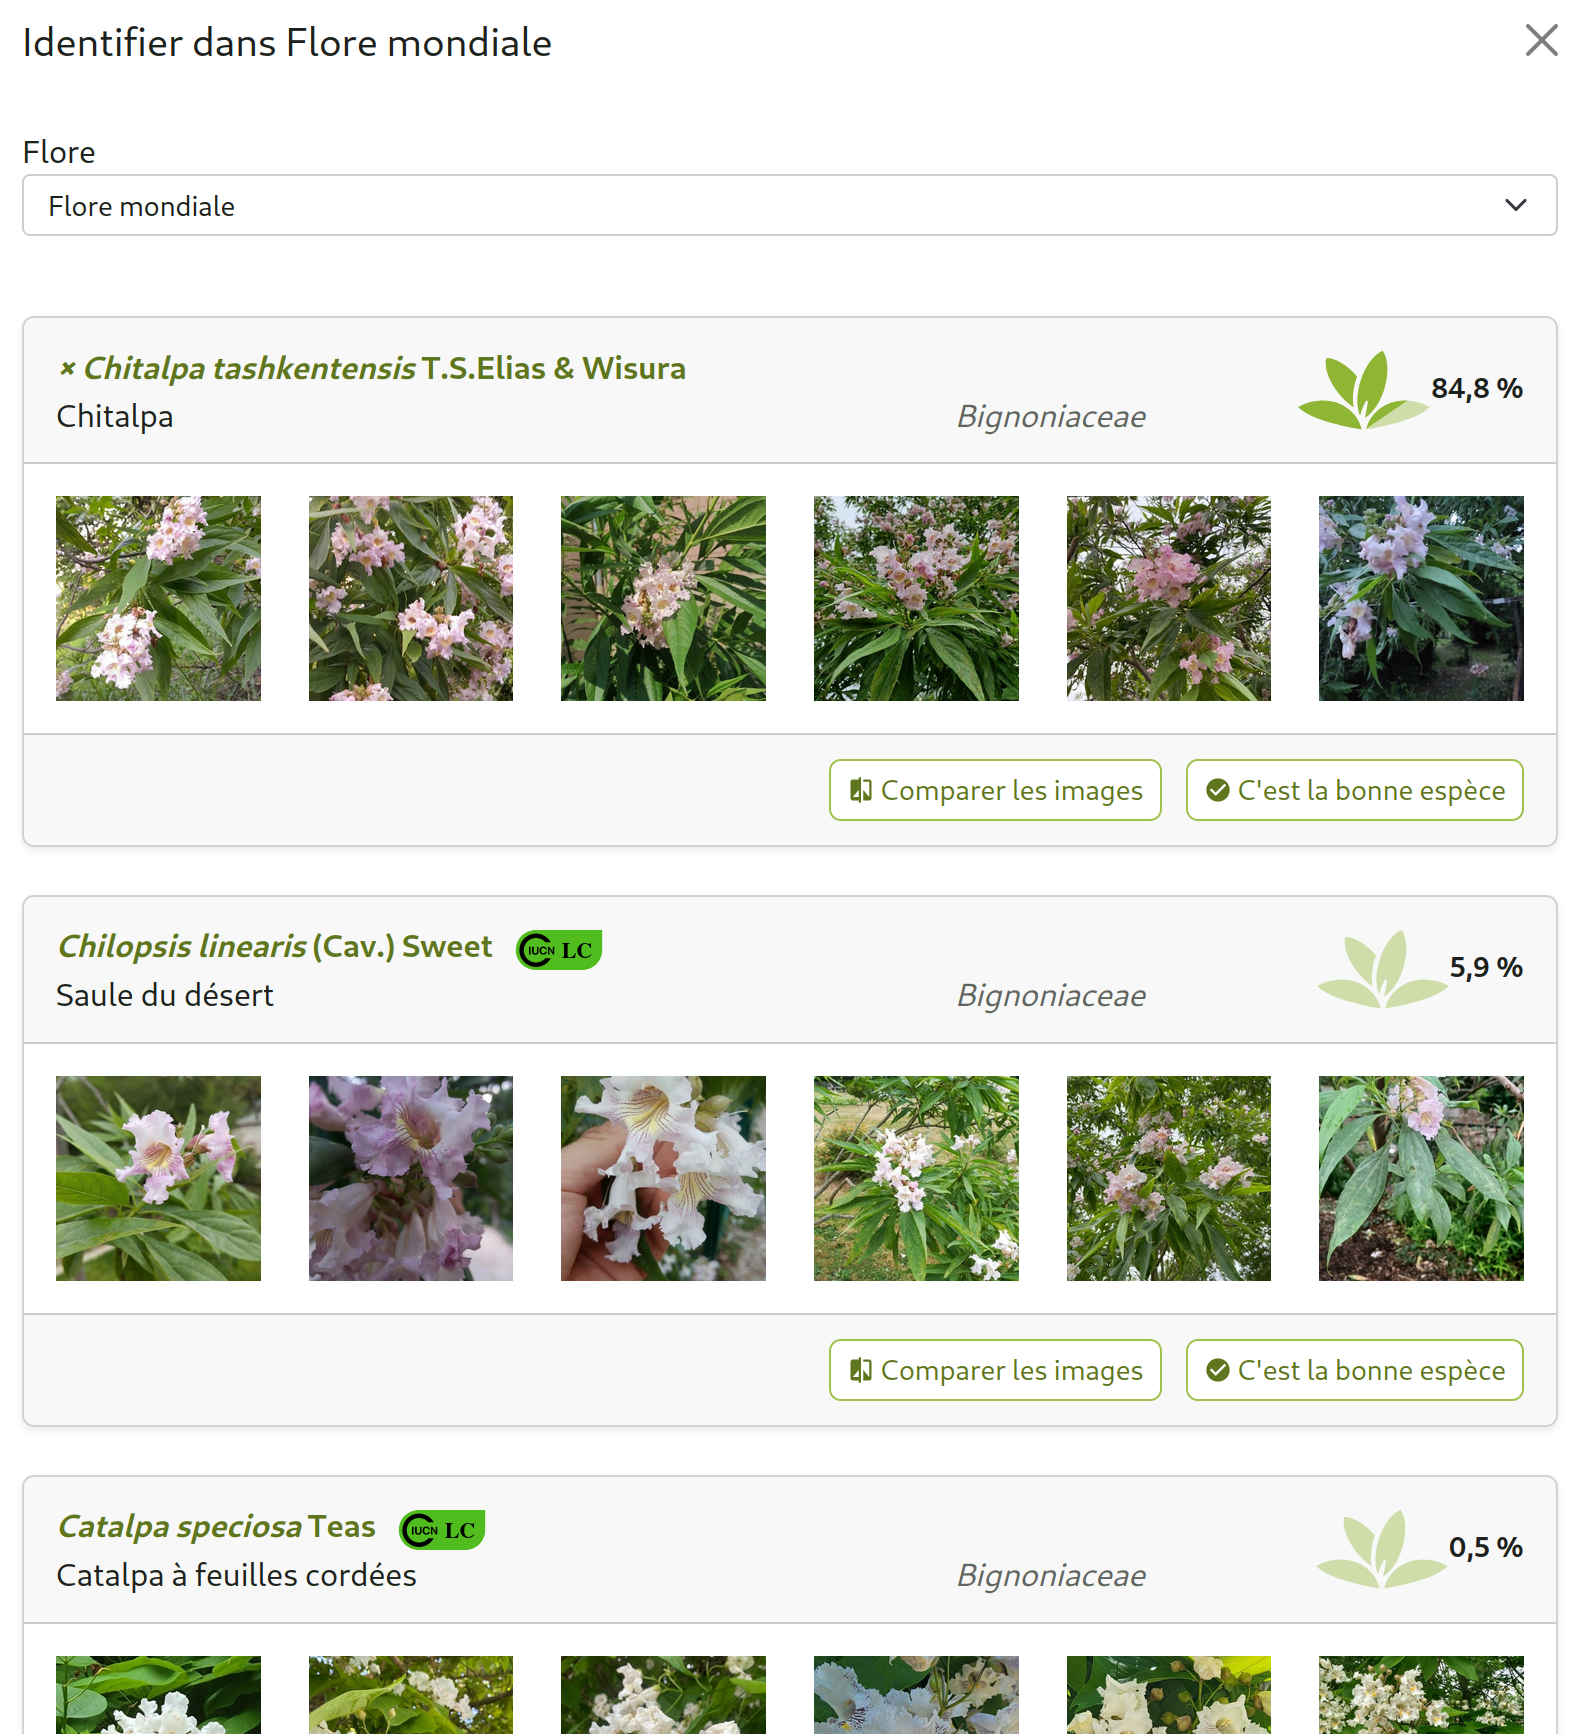
\includegraphics[width=\textwidth]{chapters/images/AI_votes.png}}
        \end{minipage}\par\medskip
            \caption{Example of observation from the Pl@ntNet online interface. The user shown is the author of the observation. We record the initial submitted species name, and the different votes (here 5 users agree on the label determination). If an observation's pictures do not contain the same plant, users can vote for a malformed label. By clicking on the icon near the identification field, users can see the current computer vision model prediction.}
    \label{fig:interface-plantnet}
\end{figure}

When voting, users are shown the current computer vision prediction on the observation -- as shown in \Cref{fig:interface-ai}. This prediction influences users' votes, but also contains information.
At the time of writing, Pl@ntNet's computer vision model is a DINOv2 \citep{oquab2024dinov2} transformer-based network.
Using contrastive learning \citep{waida2023understanding} \emph{i.e.} representing similar images as close embedding to learn similar features for similar observations and then using supervised learning to finetune the model.

In \Cref{chap:plantnet}, we present the Pl@ntNet label aggregation strategy, but also how we can incorporate model predictions into the label aggregation.
Taking into account the network's vote is a delicate matter, as we don't want the AI to become overconfident in its prediction by relying mostly on its predictions and discarding human votes.
Human expertise being the main goal of the platform, we want to keep humans in the loop, especially botanical experts to keep improving end-users plant identifications.

\subsection{Regarding ethics in crowdsourcing}
\label{sub:ethics}

Crowdsourcing tasks are useful and have led to advances in research and applications.
The issue is that not all crowdsourcing platforms have the same impact, and we know that there is still room for improvements to have more ethical crowdsourcing in general.
We do not wish or pretend in any way to provide a fully extended analysis of ethics in this area of work.
However, conducting a thesis around crowdsourced datasets without discussing worker considerations and working conditions would overlook the "where and how" the data was obtained which is not innocuous.
We only offer a discussion around the ethics that should be continued until further improvements are implemented.

As stated in \citet{schmidt2013good}, crowdsourcing and worker exploitation are closely related in practice.
Exploitation in itself is a loaded word, and we shall use the definition from \citet{mayerexploitation}:
\begin{center}
    \begin{minipage}{.75\textwidth}
    \emph{
    Exploiters, I will show, always inflict losses of a relative sort on disadvantaged parties. They do harm to their victims, even when their interactions are mutually advantageous, by failing to benefit the disadvantaged party as fairness requires.
    }
    \end{minipage}
\end{center}
Mayer further classifies the exploitation into three subsets viewed from the fairness principle:
\begin{itemize}
    \item exploiters do not benefit their victims at all,
    \item exploiters do not benefit their victims sufficiently,
    \item exploiters do not benefit their victims authentically.
\end{itemize}

In the case of part of the security system of chatgpt \citep{openai2023gpt4}, OpenAI hired the company Sama to outsource examples of potential hate speech text, violence \emph{etc.} and label them.
This labeling was done by Kenyan workers in 2021, paid between 1\$ 32 and 2\$ an hour\footnote{\url{https://time.com/6247678/openai-chatgpt-kenya-workers/}}. Here the exploiters do not benefit their victims sufficiently considering the wage\footnote{There is currently no universal minimum wage in Kenya, however in 2022 a cashier would earn in average 309.06Ksh/hour in Nairobi \emph{i.e.} around \$2.14/hour: \url{https://africapay.org/kenya/salary/minimum-wages/2182-cities-nairobi-mombasa-and-kisumu}}.

Even more recently, Toloka\footnote{\url{https://toloka.ai/}} one of the largest crowdsourcing platforms, owned by Yandex, has been found collaborating with NTechLab and Tevian -- \emph{both sanctioned under the EU's human rights regime in July 2023 for contributing to the oppression and detention of protestors in Russia}\footnote{\url{https://www.thebureauinvestigates.com/stories/2024-03-27/paid-pennies-to-train-tools-of-repression-the-humans-behind-moscows-state-surveillance/}}.
Workers were not aware of the use of their annotations when drawing bounding boxes around people in images or labeling actions from surveillance videos.
As the data was used to train facial recognition technology and employed for repression -- monitoring and detention of journalists and activists in support of Alexei Navalny for example -- the EU Council found Tevian and NTechLab to be \emph{responsible for providing technical or material support for serious human rights violations in Russia, including arbitrary arrests or detentions, and violations or abuses of freedom of peaceful assembly and of association.}\footnote{\url{https://eur-lex.europa.eu/legal-content/EN/TXT/PDF/?uri=CELEX:32023R1495}}. According to Annex I to Regulation (EU) 2020/1998, direct exchange of resources with these companies is thus prohibited and sanctioned. Further investigations are currently happening, however, the use of crowdsourcing data in this context is a clear example of possible malicious exploitations of knowledge and participation of workers.

The legal protection is also limited per the unusual working framework. At the European Union level, the Joint Research Centre (JRC) and the European Commission’s Science and knowledge service published a report\footnote{\url{https://publications.jrc.ec.europa.eu/repository/bitstream/JRC112243/jrc112243_legal_framework_digital_labour_platforms_final.pdf}} to help policymakers in their decisions stating that \emph{"current labour law framework is not aptly suited to govern new working patterns and should be revised, either on legislative or interpretative level"}.
This report stresses that \emph{"from a purely legal point of view, 'digital platform-enabled labour' does not even exist, in the sense that it is not a sort of watertight dimension of the economy and the labour market'"} as this is a very heterogeneous active field of work with difficult generalizations and conflicting perspectives between scholars, commentators and lawmakers.

Data privacy has also been of concern with the growing popularity of some platforms.
In \citet{lease2013mechanical}, Personal Identity Identification (PII) exposure factors have been identified on the Amazon Mechanical Platform -- that is considered by many as fully anonymous.
On this platform, each worker is assigned a unique identification string of both letters and numbers.
This string was provided in the final dataset and sometimes released publicly -- as a dataset or in figures as in \citet{gao2015cost}.
However, this string added to a specific URL was\footnote{currently this privacy seems to have been fixed, but it was identified in 2012 and was still active in 2019 \url{https://www.reddit.com/r/mturk/comments/bb16w8/separate_account_for_selling_on_amazon/}} the access to the worker profile.
Access to the profile meant access to names, ages, location, wish lists for purchases, and other demographic information.

Finally, we might wonder: if paid crowdsourcing brings such social and law-related issues, what about unpaid crowdsourcing -- used with Pl@ntNet?
And once again, we fall back to a case-by-case situation with the lack of regulations in this area.
New questions about vigilantism have risen with crowdsourcing platforms like BlueServo\footnote{\url{https://www.blueservo.net/}} in Texas or EuropeanBorderWatch\footnote{\url{http://www.europeanborderwatch.org/}}.
These platforms allow users to watch surveillance cameras near borders and monitor suspicious criminal activities -- immigration related mainly.
As stated in \citet{schmidt2013good}, \emph{"this
certainly brings up all kinds of ethical questions regarding the motives of those watching and reporting, the effect on those who should be paid doing these jobs and regarding those being named and shamed, potentially innocently, by a vigilant cyber mob"}.
Unpaid crowdsourcing also often comes in the form of games to keep workers in the loop and gather more data.
\citet{roglallwork} states that with this new form of labor, the risk is for workers not to be able to separate their work from these side leisure leading to problems in evaluating their working worth and compensation.
Following the classification of exploitation, the question is: does this form of unpaid work fall into one of the three subsets, does it benefit the workers?
In \citet{nystrom2021exploring}, an evaluation experiment was designed to evaluate gamified tasks: the Darkness of Gamification Evaluation System.
Previous work such as \citet{pirkkalainen2016two} identified four darkness phenomena: information overload, technostress, IT anxiety, and IT addiction.
\citet{nystrom2021exploring} concludes that gamification \emph{"could contribute to all four, thus, the designing of gamification is crucial to avoid darkness that impacts the user negatively"}.

Within this thesis, we did not conduct any new crowdsourcing experiments.
We used datasets from other research projects publicly available.
The Pl@ntNet data collection process -- explained in \Cref{chap:plantnet} -- is a form of unpaid crowdsourcing where users know that their participation helps current research (known as explicit crowdsourcing, see \Cref{chap:history-crowdsourcing} for more details).

\section{Problematic and thesis organization}

\subsection{Organization of the thesis}

In this thesis, we deal with image classification problems in crowdsourcing.
The main setting we consider is: \emph{How to learn from crowdsourced labels?}
As this is a large problem we want to focus on the data quality we learn our classifiers from, especially in a context with few labels given per task.
The literature has mainly considered modeling workers abilities and faults \citep{dawid_maximum_1979, sinha2018fast,rodrigues2018deep,raykar_ranking_2011}, but very few models incorporate the tasks' difficulty \citep{whitehill_whose_2009, chu2021learning}.
Moreover, when this difficulty is taken into account, it is often done without considering the actual images, only the answered labels \citep{whitehill_whose_2009}.
In this work, we first propose to identify ambiguous tasks in training datasets from the crowdsourced labels and the actual image with a metric called the $\mathrm{WAUM}$ introduced by \citet{lefort2022improve}.
Defining what is a difficult task proves to be a challenge in itself.
An informal definition of a difficult task is given by \citet{angelova2004data}:
\begin{center}
\begin{minipage}{.75\textwidth}
\emph{
Difficult examples are those which obstruct the learning process or mislead the learning algorithm or those which are impossible to reconcile with the rest of the examples. Defining difficult examples cannot be done without the learning model or the generating distribution.
}
\end{minipage}
\end{center}

In this work, we focus on the tempering of the learning process.
Our $\mathrm{WAUM}$ heavily relies on how easy it is for a model to learn the given task.
Furthermore, identifying possible ambiguous tasks lets us better explore large crowdsourced datasets and consider strategies to improve learning performance.
In addition, the work of \citet{merler2004bias} and more recently \citet{pleiss_identifying_2020} show significant learning performance of models after pruning most unreliable tasks from the datasets.
We show that similar improvements can be made in the crowdsourcing setting.
In \cref{chap:peerannot}, we present our open-source \texttt{python} library \texttt{peerannot} to ease and help standardize how to deal with crowdsourced datasets in image classification.
We handle label aggregation strategies, learning strategies and identification processes of ambiguous tasks and/or poorly performing workers.
We also propose a framework to evaluate multiple datasets and aggregation strategies with the \texttt{Benchopt} framework.
Finally, in \cref{chap:plantnet} we compare label aggregation strategies on a large subset of Pl@ntNet's south-western European database we released.
This subset is challenging as it contains more than $6$ million tasks and over $800$ thousand workers with a large number of classes.
We investigate Pl@ntNet's current label aggregation strategy performance and how we could improve it using the current computer vision model predictions.

\subsection{Notation}

\paragraph*{Classical supervised setting.}Let us first reconsider classical supervised learning in a classification setting.
A dataset $\mathcal{D}=\{(x_i, y_i^\star)\}_{i=1}^n$ is composed of $n$ tasks $x_i\in\mathcal{X}$ and $y_i^\star\in\mathcal{Y}$.
In image classification, $\mathcal{X}$ is classically the space of RGB images and $\mathcal{Y}$ is the set of possible labels.
The possible labels are encoded as numbers, thus in a classification problem with $K$ classes, $\mathcal{Y}=[K]=\{1,\dots,K\}$.
The cardinal of the set $\mathcal{Y}$ is written as $|\mathcal{Y}|=K$.
To classify images, we need a classifier denoted $\mathcal{C}$.
Then, given a task $x_i\in\mathcal{X}$, $\mathcal{C}(x_i)\in\mathbb{R}^K$ represents the vector of scores.
To transform these scores into probabilities, we use the softmax function $\sigma(\cdot)$ defined as:
$$
\sigma(z) = \left(\frac{e^{z_k}}{\sum_{\ell\in [K]} e^{z_\ell}}\right)_{k\in [K]} \enspace.
$$
The probabilities predicted by the classifier sorted in decreasing order are
$$
\sigma(\mathcal{C}(x_i))_{[1]} \geq \sigma(\mathcal{C}(x_i))_{[2]}\geq \dots\geq \sigma(\mathcal{C}(x_i))_{[K]} \enspace,
$$
where $\sigma(\mathcal{C}(x_i))_{[1]}$ represents the predicted class for the task by the classifier.
The indicator function is denoted $\mathds{1}(\cdot)$. The simplex of dimension $K-1$ is written as $\Delta_K=\{p \in\mathbb{R}^K_+ | \sum_{k=1}^K p_k = 1\}$.
And finally, given a vector $z\in\mathbb{R}^K$, we denote the normalization operator $\mathbf{N}$ such that $\mathbf{N}(z) = z / \sum_{k\in[K]}z_k$.

\begin{figure}[thb]
    \centering
    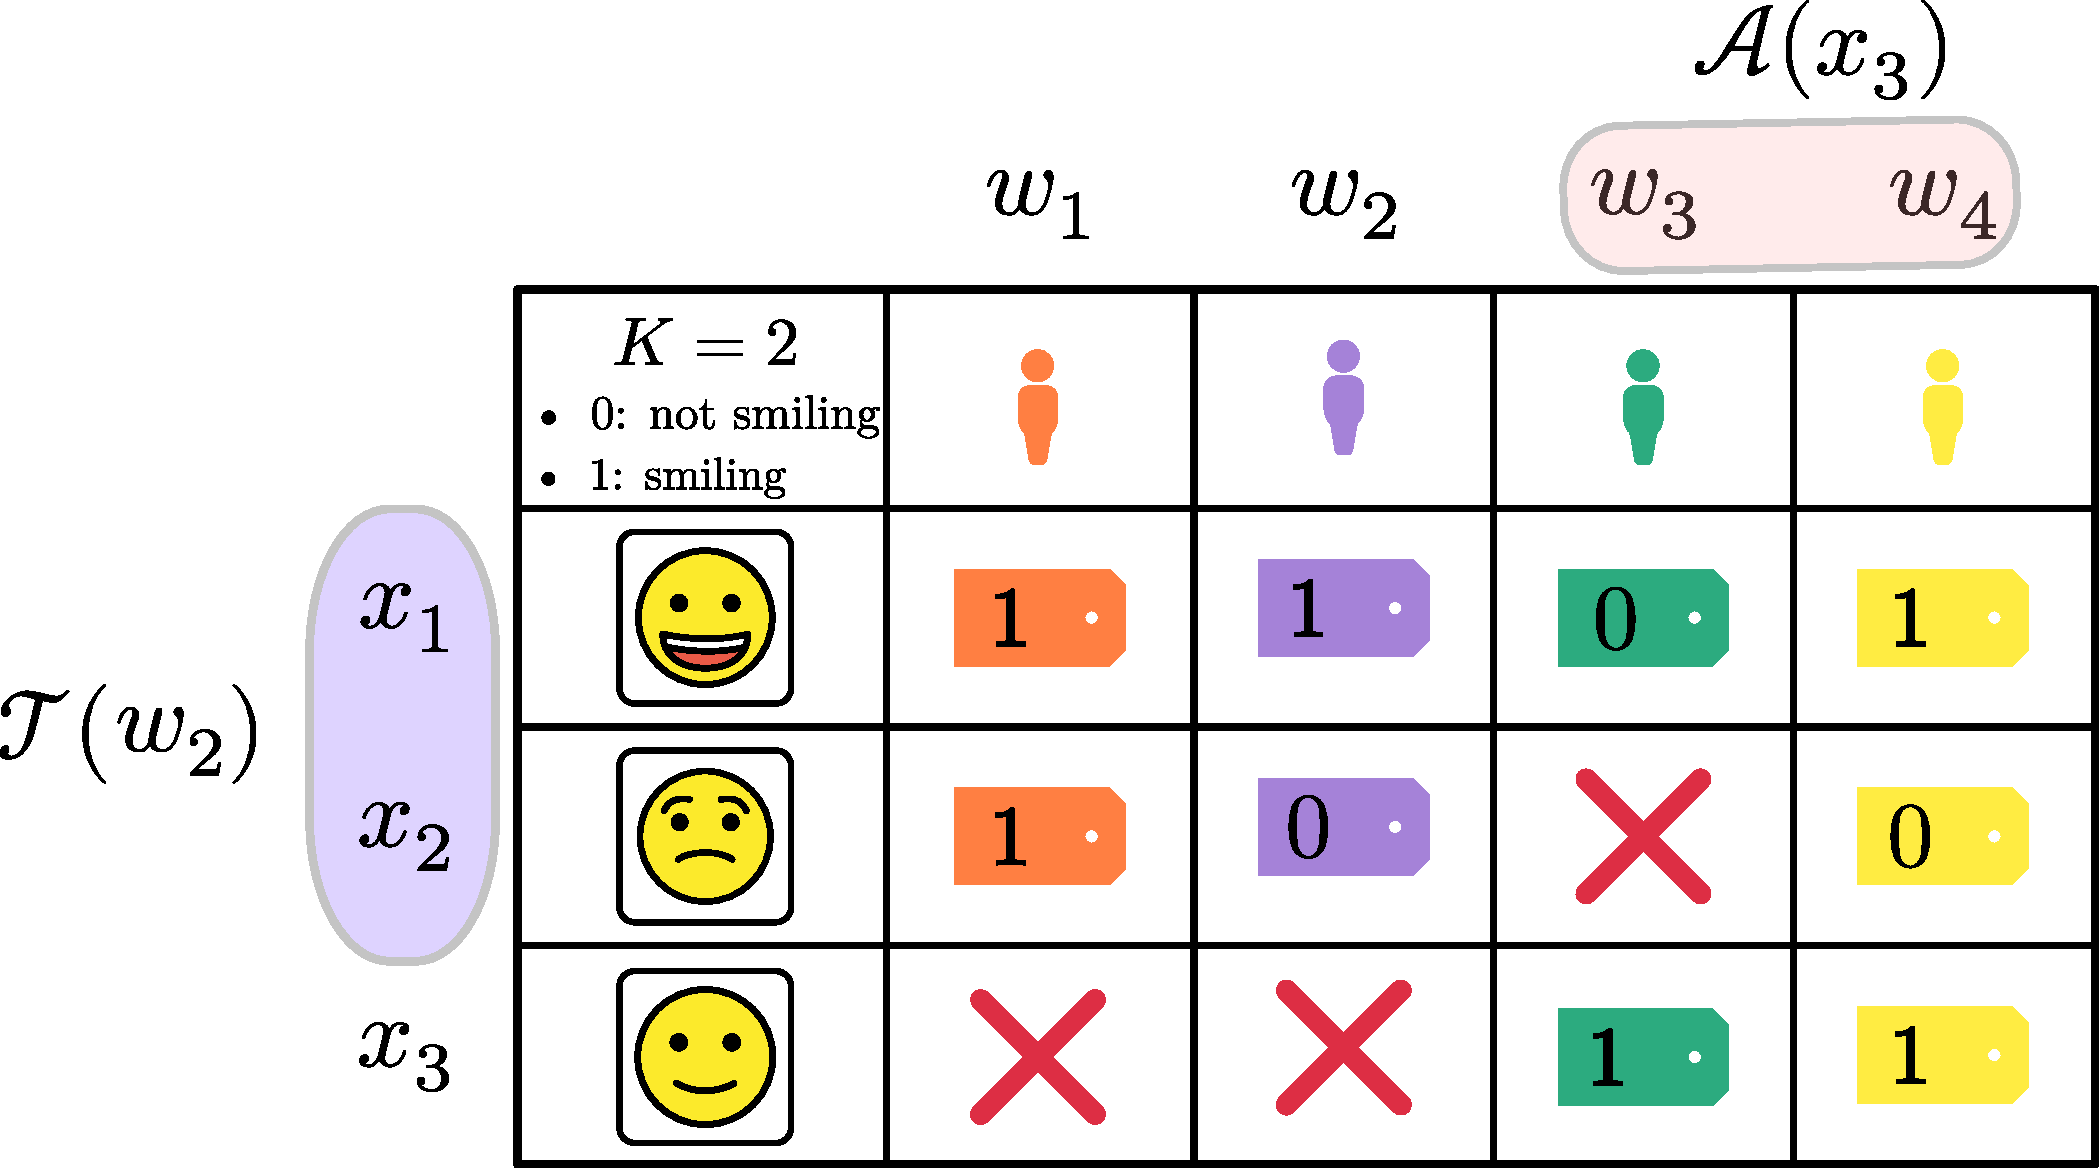
\includegraphics[width=.7\textwidth]{chapters/images/notations.pdf}
    \caption{Crowdsourcing notation on a toy example. There are three tasks to classify into $K=2$ groups. Only worker $w_4$ answers all tasks. Only the task $x_1$ is answered by all workers. The workerload of $w_2$ is $|\mathcal{T}(w_2)|=|\{1,2\}|=2$. The feedback effort on $x_3$ is $|\mathcal{A}(x_3)|=|\{3,4\}|=2$.}
    \label{fig:enter-label}
\end{figure}

\paragraph*{Crowdsourcing setting.}
With crowdsourced data, the ground truth $y_i^\star$ of a task $x_i$ is unknown.
Instead, there is a crowd of $n_{\text{worker}}\in \mathbb{N}^\star$ labeling the $n_\text{task}$ training tasks -- we assume access to a classical test and validation set.
Each worker $w_j,j\in [n_{\text{worker}}]$ answers at least one task by giving a label denoted $y_i^{(j)}\in[K]$.
The set of workers answering the task $x_i$ is denoted by
\begin{equation}\label{eq:feedback}
\mathcal{A}(x_i)=\left\{j\in[n_\text{worker}]: w_j \text{ answered }x_i\right\}.
\end{equation}
We call \textbf{feedback effort} the number of labels for a given task: $|\mathcal{A}(x_i)|$.
Note that the feedback effort can not exceed the total number of workers $n_{\text{worker}}$.

Similarly, one can adopt a worker point of view: the set of tasks answered by a worker $w_j$ is denoted
\begin{equation}\label{eq:workerload}
\mathcal{T}(w_j)=\left\{i\in[n_\text{task}]: w_j \text{ answered } x_i\right\}.
\end{equation}
The cardinal $\vert \mathcal{T}(w_j)\vert$ is called the \textbf{workerload} of $w_j$.
The final dataset can then be decomposed as:
\begin{equation}\label{eq:trainset}
\mathcal{D}_{\text{train}} := \bigcup_{i\in[n_\text{task}]} \left\{(x_i, (y_i^{(j)})) \text{ for }j\in\mathcal{A}(x_i)\right\} = \bigcup_{j\in[n_\text{worker}]} \left\{(x_i, (y_i^{(j)})) \text{ for }i \in\mathcal{T}(w_j)\right\} .
\end{equation}
Note that we use the index notation $i$ for the tasks and $j$ for the workers in the crowdsourcing experiments.

\subsection{Existing label aggregation strategies}
\label{sub:aggregating_votes}

\begin{figure}[ht]
    \centering
    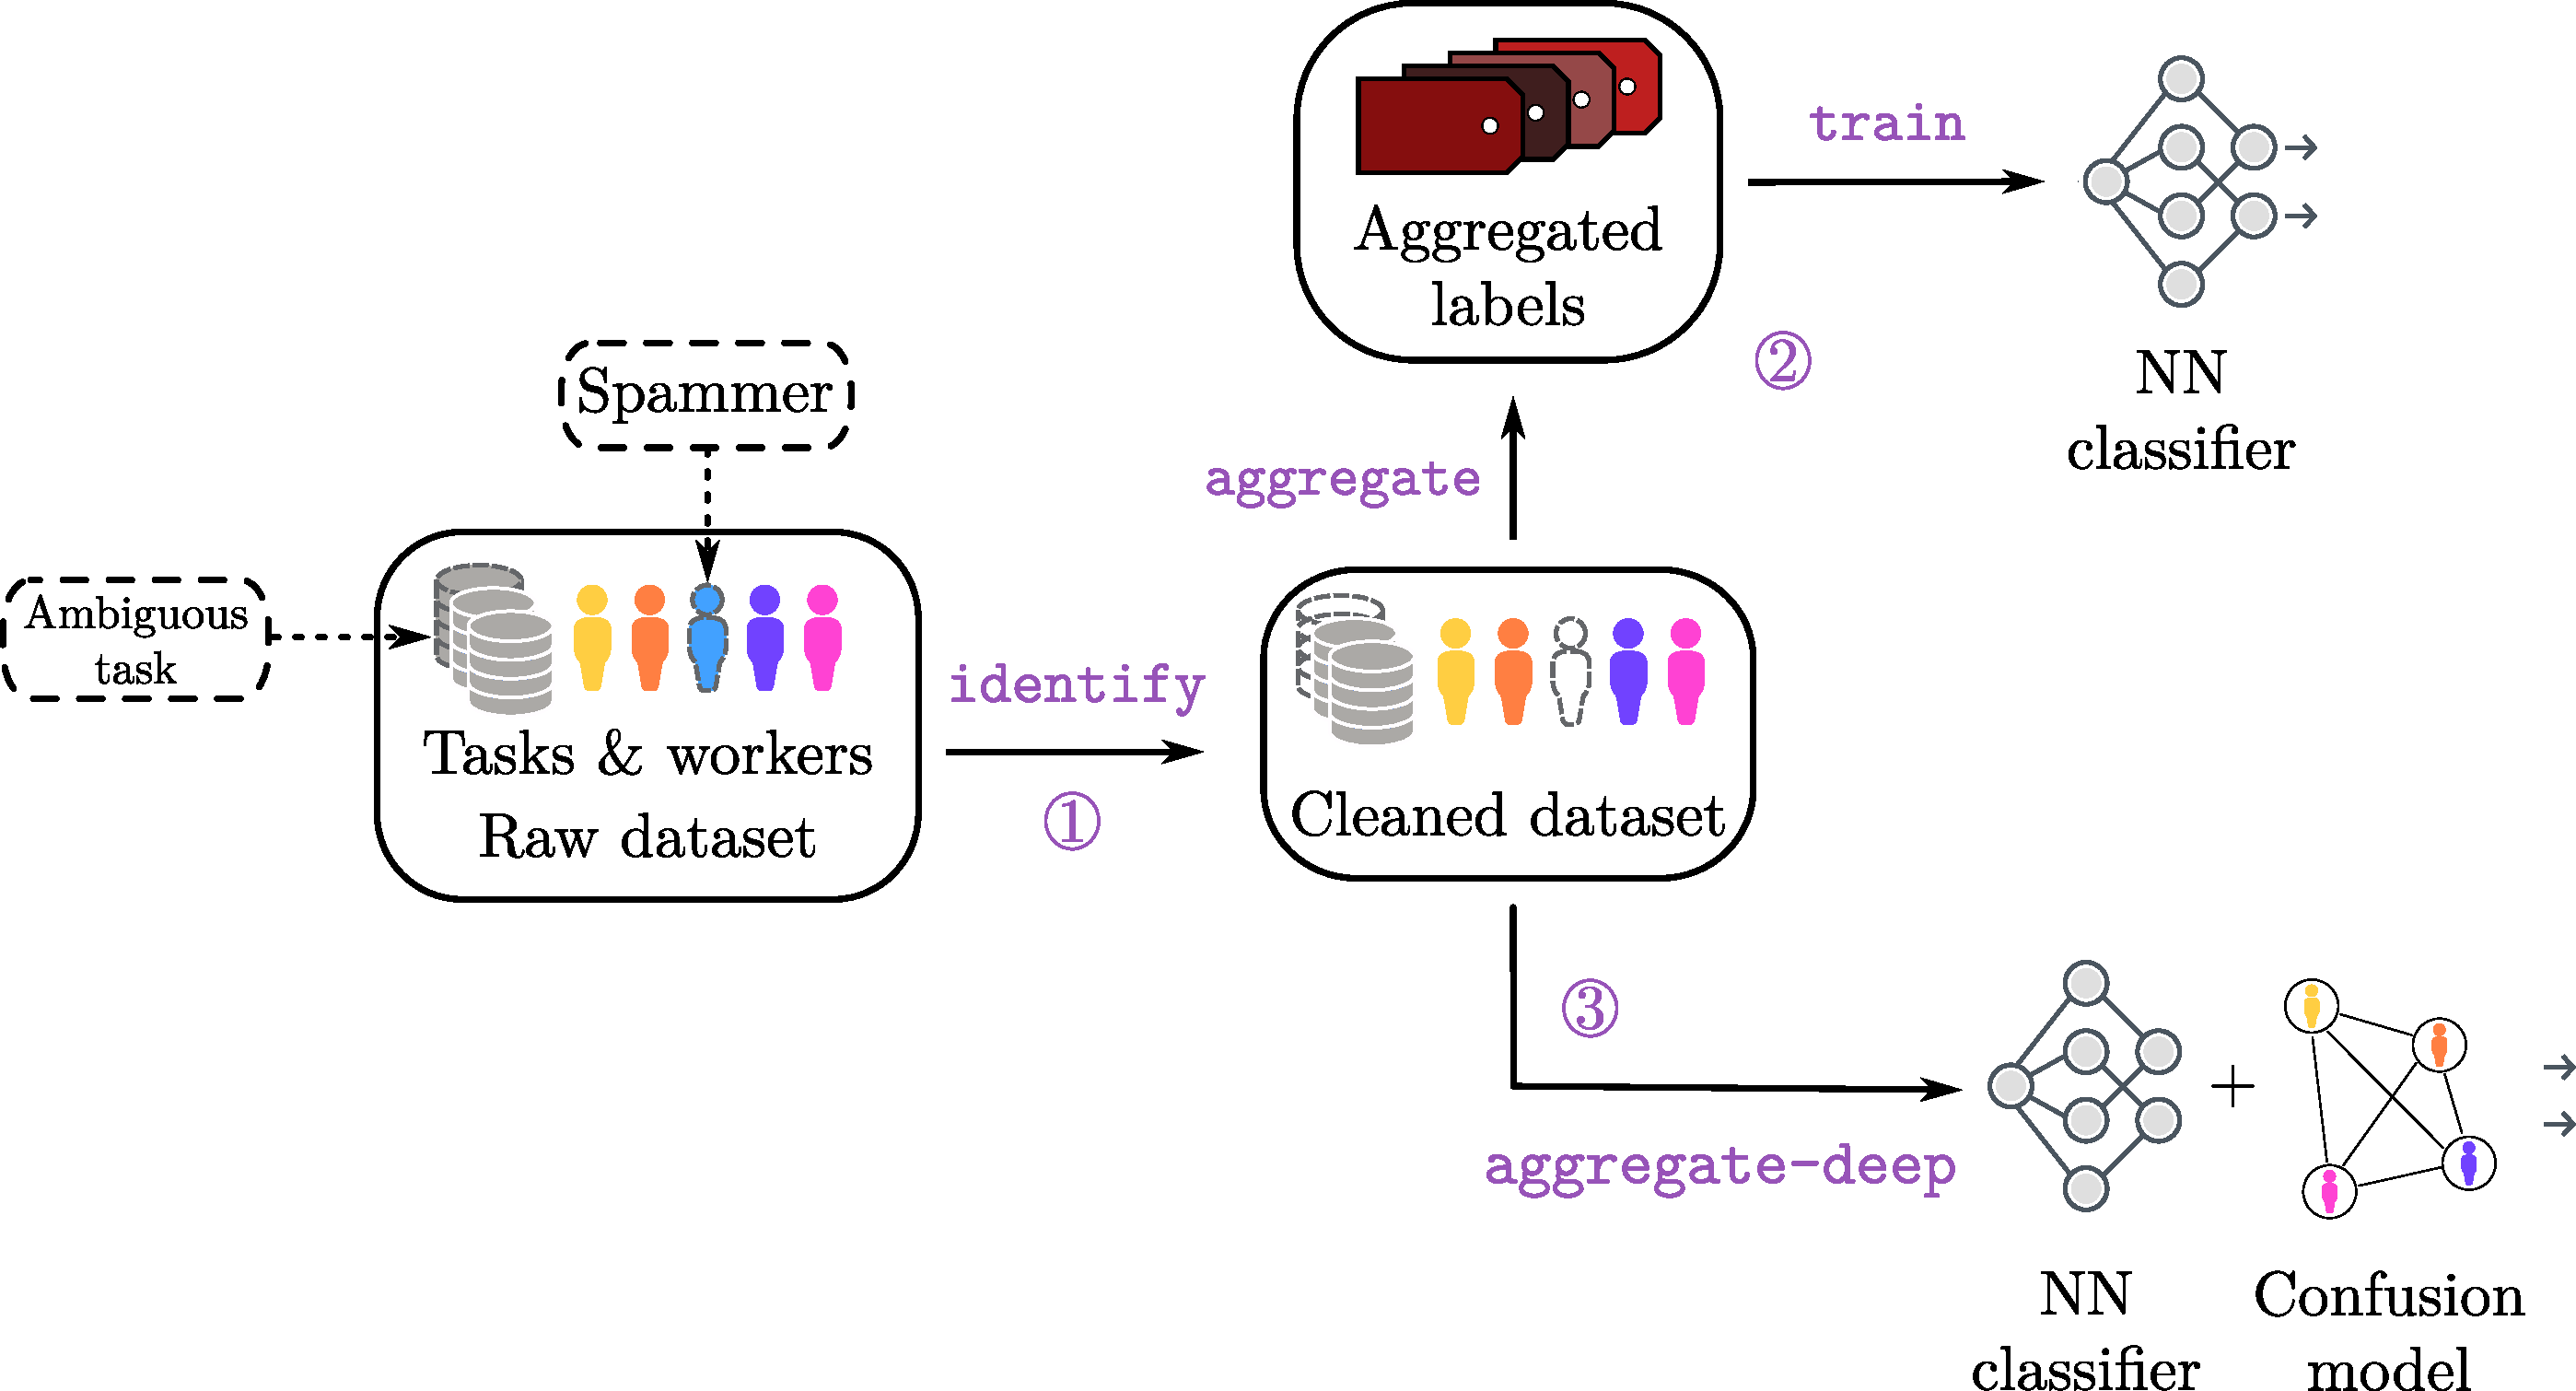
\includegraphics[width=\textwidth]{chapters/images/strategies_crowd_data.pdf}
    \caption{pipleine of crowdsourcing experiments. The data is collected. We identify poorly performing workers and/or ambiguous tasks. Then labels are aggregated to be used in a supervised learning setting. If the tasks are available and the goal is to learn a predictor, deep-learning-based strategies can be used to learn the confusion model and the classifier at the same time.}
    \label{fig:pipeline_crowdsourcing}
\end{figure}

If the goal of the crowdsourcing experiment is to associate a label with a task in the training set, then we need to aggregate the collected labels into a single one.
This aggregation step can lead to two types of labels:
\begin{itemize}
    \item hard labels: the aggregated label $\hat y_i\in [K]$ represents a single class -- it can be seen as a Dirac distribution over $\mathcal{Y}$.
    \item soft labels: the aggregated label $\hat y_i\in\Delta_K$ is a probability distribution over $\mathcal{Y}$ that is not necessarily a Dirac. This type of label keeps more of the uncertainty for the learning procedure.
\end{itemize}
Note that if the aggregation step produces a soft label, it is always possible to produce a hard label taking the mode of the distribution -- \emph{i.e.} using the $\mathrm{argmax}$ function.

In the following, we present classical aggregation strategies.
This is not an exhaustive list, only models we mostly use for comparison.
Assume that a dataset $\left(x_i, \{y_i^{(j)}\}_{j\in\mathcal{A}(x_i)}\right)_{i\in [n_\text{task}]}$ is available.
We only need to consider the proposed labels -- \emph{i.e.} the tasks $x_i$ are not used.
These models -- and more -- are available in the library \texttt{peerannot} using the \texttt{aggregate} command shown in \Cref{fig:pipeline_crowdsourcing}.

\subsubsection{Majority vote (MV)}
\label{subsub:mv}

The majority vote strategy is the simplest mechanism to create a label from multiple answers.
It consists in collecting the votes and taking the most answered category.
In the case of a draw, a random choice in the most answered choices is applied.
More formally:

\begin{equation}\label{eq:mv}
    \forall i\in [n_\text{task}],\ \hat y_i^{\mathrm{MV}} = \underset{k\in[K]}{\mathrm{argmax}}\left(\sum_{j\in\mathcal{A}(x_i)} \mathds{1}(y_i^{(j)}=k)\right)_{k\in[K]} \enspace.
\end{equation}

The main drawback of the majority vote is the lack of consideration of workers' abilities.
Intrinsically, this aggregation strategy assumes that all workers are equal.
However, experiments have shown that this is not true \citep{snow_cheap_2008,vuurens2011much}.
The MV strategy is one of the most theoretically studied thanks to its simplicity.
\citet{wang2015crowdsourcing} found that the label error rate decreases exponentially with the number of workers selected for each task. This assumes that the worker quality is bounded and the workers are selected uniformly in the crowd.
In the same work, they also provide similar results with worker quality characterized by their specificity -- true negative rate -- and sensitivity -- true positive rate -- with Gaussian-like assumptions instead of bounded qualities.
Another issue with the MV strategy is that by taking the mode of the votes' distribution, the labeling uncertainty completely disappears (see \Cref{fig:confusion-types}).

\begin{figure}[htb]
    \centering
    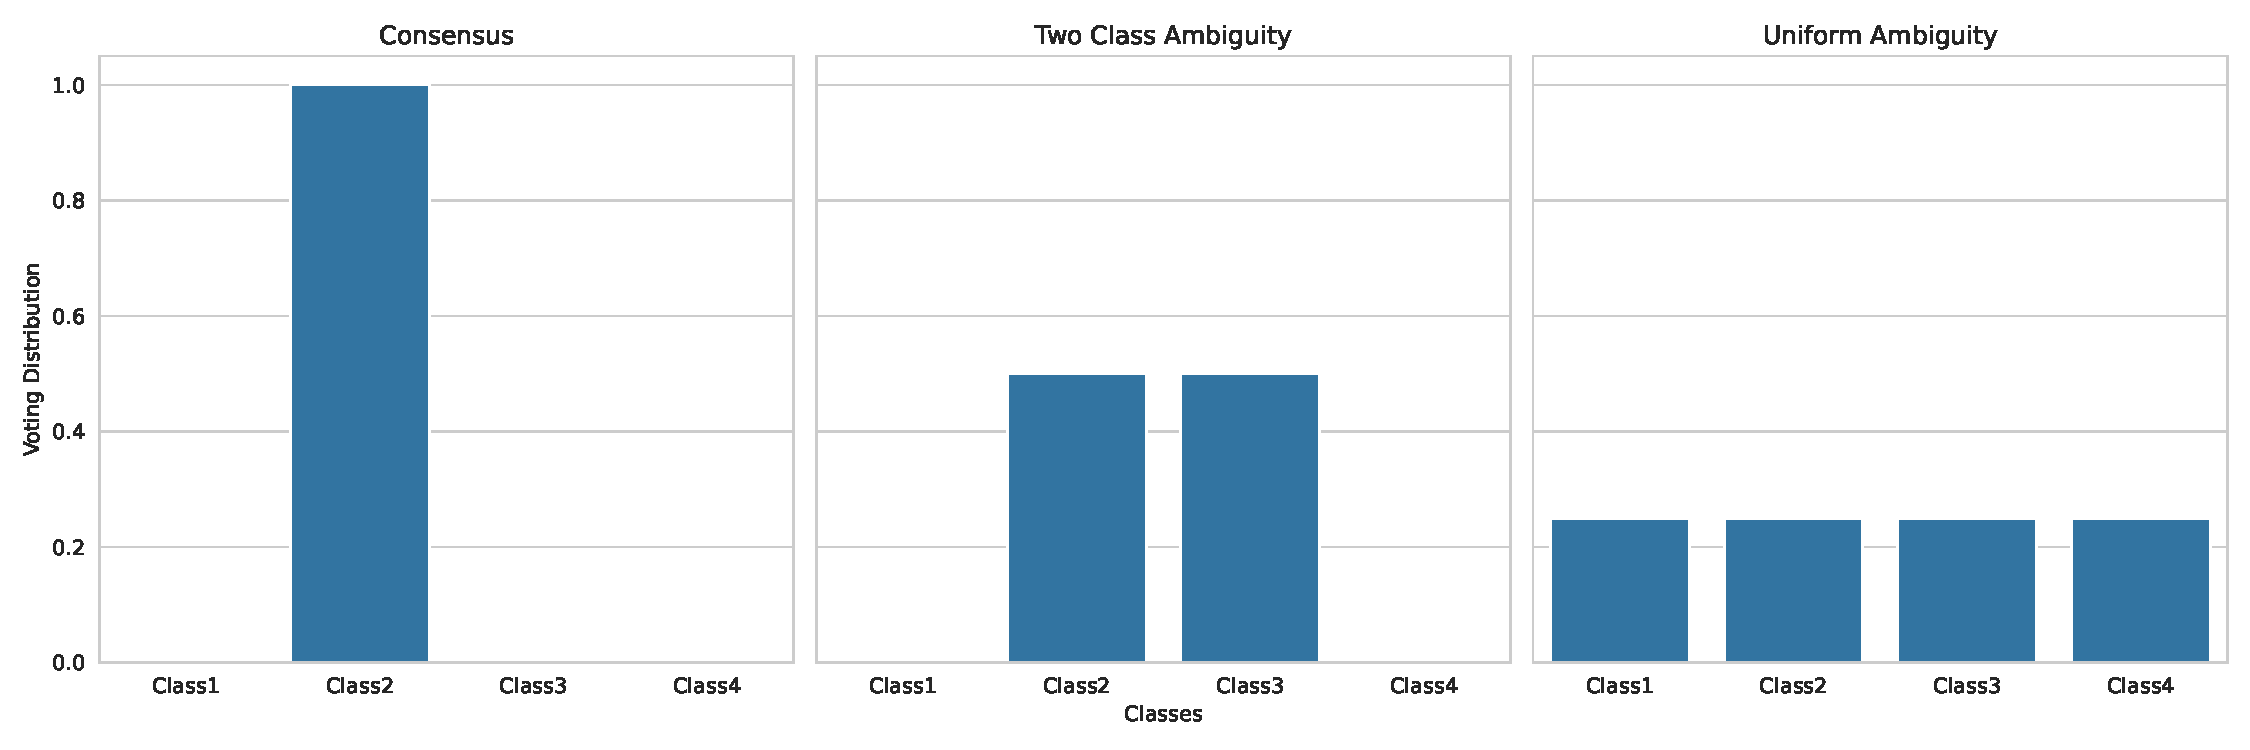
\includegraphics[width=.96\textwidth]{chapters/images/ambiguity.pdf}
    \caption{Three different configurations where the MV strategy can lead to the same label. When there is consensus there is no ambiguity to select the label. However, ambiguities can happen differently. There can be ambiguities between all classes or between a subset of classes.}
    \label{fig:confusion-types}
\end{figure}

Furthermore, the majority vote is sensitive to a specific type of attack on the data: \textbf{spams}.
A spammer is defined as a worker whose answers are given independently of the underlying ground truth \citep{raykar_ranking_2011}. More formally:
\begin{equation}\label{eq:spammer}
    \forall i \in [n_\text{task}] \forall (k,c) \in [K]^2,\ \mathbb{P}(y_i^{(j)} = k\ | y_i^\star=c) = \mathbb{P}(y_i^{(j)} = k) \enspace.
\end{equation}
\citet{vuurens2011much} discusses how critical it is to identify spammers to improve labeling quality. They show through several simulation settings that even with trapping systems, the majority vote is still susceptible to spam.

In practice, the MV strategy is most often used as a baseline strategy.
Note that some taskmasters improved majority vote accuracy using prevention systems that are not considered throughout this work.
\citet{hoang2021tournesol} for example uses a vouching system where volunteer workers can be approved via specific institutional email domains.
\citet{khattak_toward_2017} and \citet{peterson_human_2019} use trapping sets -- \emph{i.e.} separate set of tasks where a ground truth is known. This set is considered to evaluate worker abilities and identify poorly performing workers, or potential spammers. \citet{vuurens2011much} showed that these sets lead to still sensitive decisions regarding other types of spammers.

\subsubsection{Naive Soft (NS)}
\label{subsub:ns}

To compensate for the loss of uncertainty of the MV strategy, the simplest solution is not to consider the mode of the voting distribution but to keep the full distribution as a label.
The Naive Soft (NS) strategy creates a simple soft label in the simplex from the frequency of votes for each class.
\begin{equation}\label{eq:ns}
    \forall i\in [n_\text{task}],\ \hat y_i^{\mathrm{NS}} = \mathbf{N}\left(\sum_{j\in\mathcal{A}(x_i)} \mathds{1}(y_i^{(j)}=k)\right)_{k\in[K]} \enspace.
\end{equation}

Recent work \citep{collins2022eliciting} showed that with enough votes collected, naive soft labels do lead in general to better probability outputs in predictions (in terms of calibration error -- see the $\mathrm{ECE}$ error in \Cref{sub:evaluation-metrics} for more details) compared to hard labels.
However, this strategy still considers every worker equal in front of the tasks proposed like the MV, thus does not alleviate any ability score, for example not to be corrupted by spammers.

\subsubsection{Dawid and Skene (DS)}
\label{subsub:ds}

The Dawid and Skene's (DS) strategy \citep{dawid_maximum_1979} introduced a framework where each worker is represented by its confusion.
This way, it is the first strategy to take into account worker abilities for each possible class.
Through their model, they estimate simultaneously the worker confusion and the tasks' soft label.
With its theoretical guarantees \citep{gao2013minimax} and its flexibility in the sense that it is easy to modify it to take into account data specificities \citep{passonneau-carpenter-2014-benefits, servajean2017crowdsourcing,sinha2018fast}, the DS strategy remains a strong competitor in many cases.

\begin{figure}[htb]
    \centering
    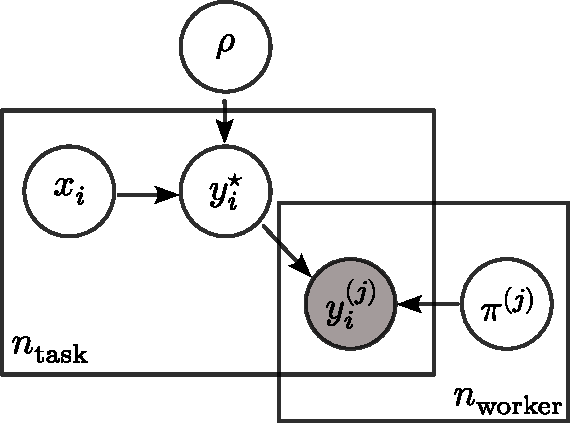
\includegraphics[width=.65\textwidth]{chapters/images/bayesien_plaque_ds.pdf}
    \caption{Bayesian plate diagram representation of the DS model. Only the labels $\{y_i^{(j)}\}_{i,j}$ are observed. Latent variables to estimate are the true labels $(y_i^\star)_i$, the prevalence $\rho$ of each class and the confusion matrices $\{\pi^{(j)}\}_j$ for each worker. The underlying task features $(x_i)_i$ are not considered.}
    \label{fig:plaque_ds}
\end{figure}

The model keystone of the DS model is the modeling of the workers' answers.
Each worker is associated to its confusion matrix $\pi^{(j)}\in\mathbb{R}^{K\times K}$ such that the $(k,\ell)$-entry represents the probability for worker $w_j$ to answer $\ell\in[K]$ when the ground truth is $k\in[K]$.
Then, we assume that each worker's answer is drawn from a multinomial distribution over the $k^{th}$ row of its confusion matrix.
More formally:
\begin{equation}\label{eq:ds_multinomial}
    (y_i^{(j)}\ | y_i^\star = k) \sim \mathcal{M}\left(\pi^{(j)}_{k,\cdot}\right)
\end{equation}

Given the probabilistic model, we wish to maximize the likelihood concerning the confusion matrices, the prevalence of each class in the dataset and the underlying true labels.
Assume that the ground truths are sampled from a multinomial distribution parameterized by the class prevalence $\rho\in\Delta_K$ -- $\emph{i.e.}$ for $k\in[K]$, $\mathbb{P}(y_i^\star=k)=\rho_k$, and that workers answer independently from one another.
Denote $T_{i,k}=\mathds{1}(y_i^\star=k)$ the indicator of the true label.
Then the maximum likelihood estimation of the DS model writes:
\begin{equation}\label{eq:ds_likelihood}
\argmax_{\rho,\pi,T}\displaystyle\prod_{i\in [n_{\texttt{task}}]}\prod_{k \in [K]}\bigg[\rho_k\prod_{j\in [n_{\texttt{worker}}]}
    \prod_{\ell\in [K]}\big(\pi^{(j)}_{k, \ell}\big)^{\mathds{1}_{\{y_i^{(j)}=\ell\}}}
    \bigg]^{T_{i,k}} \enspace.
\end{equation}

\begin{constructionbox}[Construction of the DS likelihood]
Given a single task $i$ with true label $y_i^\star=k$ and one worker $w_j$, then responses of worker $j$ follow a multinomial distribution by \Cref{eq:ds_multinomial} and the likelihood of the observed data $\{y_i^{(j)}\}_{i,j}$ is proportional to:
\begin{equation*}
    \prod_{\ell\in[K]}\left(\pi^{(j)}_{k,\ell}\right)^{\mathds{1}_{\{y_i^{(j)}=\ell\}}} \enspace.
\end{equation*}
Then, conditionally on the true label being $k$ -- \emph{i.e.} $T_{i,k}=1$ and for $k'\neq k$, $T_{i,k'}=0$, we can use the workers' independence assumption to consider multiple workers:
\begin{equation*}
    \prod_{j\in [n_{\text{worker}}]}\prod_{\ell\in[K]}\left(\pi^{(j)}_{k,\ell}\right)^{\mathds{1}_{\{y_i^{(j)}=\ell\}}} \enspace.
\end{equation*}
Removing the conditional assumption on the true label, we take into account the class prior contained in the prevalence vector $\rho$:
\begin{equation*}
    \prod_{k\in[K]} \left[\rho_k\prod_{j\in [n_{\text{worker}}]}\prod_{\ell\in[K]}\left(\pi^{(j)}_{k,\ell}\right)^{\mathds{1}_{\{y_i^{(j)}=\ell\}}}\right]^{T_{i,k}} \enspace.
\end{equation*}
Finally, as all tasks are independent, we obtain \Cref{eq:ds_likelihood} by multiplying over the task index.
\end{constructionbox}

Note that the likelihood in \Cref{eq:ds_likelihood} can not be maximized directly.
Using the expectation-maximization (EM) algorithm \citep{Dempster_Laird_Rubin77}, we can define a recursive procedure to estimate $\rho,\pi=\{\pi^{(j)}\}_j$ and $T=\{T_{i,k}\}_{i,k}$.
\begin{itemize}
    \item Assuming that $T$ is known, compute $\rho$ and $\pi$.
    \item Assuming that $\rho$ and $\pi$ are known, compute $T$.
\end{itemize}

\paragraph{With $T$ known: }
Denote $Y=\{y_i^{(j)}\}_{i,j}$ for readability.
The logarithm of the likelihood function writes:
\begin{equation*}
    \log \text{Lik}(\pi,\rho|T, Y) = \sum_{i} \sum_{k} \left[T_{i,k} \log (\rho_k) \sum_j \sum_\ell \mathds{1}_{\{y_i^{(j)}=\ell\}}\log(\pi^{(j)}_{k,\ell})\right] \enspace.
\end{equation*}
To compute $\pi$ and $\rho$ knowing $T$, we use the Lagrangian multipliers method. Let $\lambda=\{\lambda^{(j)}\}_{j}$ the Lagrange multipliers for the constraint $\sum_\ell \pi_{k,\ell}^{(j)}=1$ -- sum of probabilities for each row of confusion matrices equals $1$ -- and $\eta$ the Lagrange multiplier for the constraint $\sum_k \rho_k=1$ -- the prevalence must sum to $1$. Then the full Lagrangian $\mathcal{L}$ writes:
\begin{equation*}
        \mathcal{L}(\pi,\rho,\lambda,\eta) = \log \text{Lik}(\pi,\rho|T, Y)  + \eta\sum_i \left[\sum_k T_{i,k} \log(\rho_k) - 1\right]
        + \sum_j \lambda_{j}\sum_\ell\left[\pi^{(j)}_{k,\ell} - 1\right]
        \enspace.
\end{equation*}

\begin{itemize}
    \item Differentiation with respect to $\pi^{(j)}_{k,\ell}, (k,\ell)\in[K]^2$:
    \begin{equation*}
        \frac{\partial \mathcal{L}}{\partial \pi^{(j)}_{k,\ell}} = \sum_i \frac{T_{i,k}}{\pi^{(j)}_{k,\ell}} \mathds{1}_{\{y_i^{(j)}=\ell\}} - \lambda_j \enspace,
    \end{equation*}
    and setting it to zero leads to:
        \begin{equation}\label{eq:em_pi}
       \pi^{(j)}_{k,\ell} = \frac{1}{\lambda_j}\sum_i T_{i,k}\mathds{1}_{\{y_i^{(j)}=\ell\}}\enspace.
    \end{equation}
    \item Differentiation with respect to $\rho_k, k\in[K]$:
    \begin{equation*}
        \frac{\partial \mathcal{L}}{\partial \rho_k} = \sum_{i}\frac{T_{i,k}}{\rho_k} - \eta\enspace,
    \end{equation*}
    and setting the derivative to zero leads to:
    \begin{equation}\label{eq:em_rho}
        \rho_k = \frac{1}{\eta} \sum_i T_{i,k} \enspace.
    \end{equation}
    \item Differentiating with respect to $\lambda_j$ and $\eta$ recovers the constraints conditions.
    Taking into account the constraints we finally obtain:
    \begin{equation}\label{eq:constraints_em_ds}
        \lambda_j = \sum_{\ell'} \sum_i T_{i,k} \mathds{1}_{\{y_i^{(j)}=\ell'\}} \quad \text{and}\quad \eta = n_{\text{task}}
    \end{equation}
\end{itemize}
Combining \Cref{eq:constraints_em_ds} with \Cref{eq:em_pi} and \Cref{eq:em_rho}, we obtain the update rule for $\pi$ and $\rho$ with $T$ known.

\paragraph{Update rule for $T$: }We now estimate $T$ with $\pi$ and $\rho$ known using Bayes formula. Recall that $T_{i,k}$ represents the posterior probability of task $i$ to belong in class $k$ given the observed labels $Y$, the class prevalence $\rho$ and the confusions $\pi$. Then:
\begin{align}\label{eq:ds_update_T}
    \mathbb{P}(T_{i,k}=1|Y,\pi,\rho)
    & \propto \mathbb{P}(Y,T_{i,k}=1|\pi,\rho) \notag\\
    & \propto  \mathbb{P}(T_{i,k}=1|\rho) \mathbb{P}(\{y_i^{(j)}\}_j|\pi, T_{i,k}=1) \notag\\
    & \propto \rho_k \prod_j\prod_\ell \left(\pi^{(j)}_{k,\ell}\right)^{\mathds{1}_{\{y_i^{(j)}=\ell\}}} \enspace.
\end{align}

Using our updates rules, we can now write the full EM optimization for the DS model in \Cref{alg:ds}.

\begin{algorithm}
\caption{Expectation-Maximization (EM) for Dawid and Skene Model}
\label{alg:ds}
\begin{algorithmic}[1]
\STATE Initialize $T$ with NS strategy
\WHILE{Not converged}
    \STATE // M-step: Maximization step
    \FOR{$k = 1$ to $K$}
        \FOR{$\ell = 1$ to $K$}
            \STATE Update $\pi_{k,\ell}$ using \Cref{eq:em_pi}
        \ENDFOR
        \STATE Update $\rho_k$ using \Cref{eq:em_rho}
    \ENDFOR

    \STATE Normalize $P(T_{i,\cdot} = 1 | Y, \pi, \rho)$
    \STATE // E-step: Expectation step
    \FOR{$i = 1$ to $n_{\text{task}}$}
        \FOR{$k = 1$ to $K$}
            \STATE Compute posterior $P(T_{ik} = 1 | y, \pi, \rho)$ using \Cref{eq:ds_update_T}
        \ENDFOR
    \ENDFOR
\ENDWHILE
\end{algorithmic}
\end{algorithm}

At this point, a few clarifications are needed for \Cref{alg:ds}.
The initialization used for the estimated labels $T$ is the NS strategy \Cref{sub:aggregating_votes} \Cpageref{subsub:ns}, however, other initialization exist and are discussed in \citet{dawid_maximum_1979}.
Numerically, as there is no single optimum, discrepancies in results might happen.
Furthermore, let us discuss the stopping criterion.
Given a precision $\epsilon>0$, a possible criterion to stop is if, between two consecutive iterates, the likelihood did not go further than $\epsilon$ in absolute value.
Other criteria could be applied, like relative error instead of absolute, but often do not impact results by much.

\subsubsection{Weighted with Dawid and Skene (WDS)}
\label{subsub:wds}

The DS model, by design, often leads to soft labels $(T_{i,\cdot})_i$ with very low entropy distribution.
Indeed, this variable represents the indicator function of belonging to a given class.
To keep more uncertainty, one possibility is to shift our focus to only consider the diagonal of the confusion matrices estimated in the DS model.
Each term on the diagonal represents the ability of the worker to answer correctly the underlying label.
Using this DS diagonal, we obtain a weighted majority vote denoted WDS:

\begin{equation}
    \hat y_i^{\mathrm{WDS}} = \left(\sum_{j\in\mathcal{A}(x_i)} \pi^{(j)}_{k,k}\mathds{1}_{\{y_i^{(j)}=k\}}\right)_{k\in[K]} \enspace.
\end{equation}

\subsubsection{Generative model of Labels, Abilities, and Difficulties (GLAD)}
\label{subsub:glad}

\begin{figure}[thb]
    \centering
    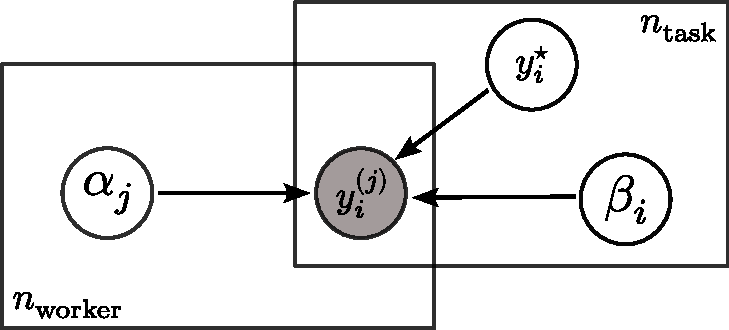
\includegraphics[width=.6\linewidth]{chapters/images/glad_plaque.pdf}
    \caption{Bayesian plate diagram representation of the GLAD model. Only the labels $\{y_i^{(j)}\}_{i,j}$ are observed. Parameters to estimate are the true labels $(y_i^\star)_i$, the worker ability $\alpha_j$ and the task difficulty $\beta_i$. The underlying task features $(x_i)_i$ are not considered.}
    \label{fig:plaque_glad}
\end{figure}

While DS-like models focused on evaluating workers' confusion, \citet{whitehill_whose_2009} introduced GLAD to take into account two sources of error: the worker's ability and the task's difficulty.
The worker ability is defined as a parameter $\alpha_j\in\mathbb{R}$. The larger the more reliable a worker is.
When $\alpha_j = 0$, the worker answers randomly, whereas when $\alpha_j<0$, the worker is adversarial and switches labels.
The task difficulty is denoted using the parameter $\beta_i\in\mathbb{R}^\star_+$.
If $\beta_i\simeq 0$, the task is almost impossible to classify correctly. When $\beta_i$ is large, the task is easy to classify.
GLAD's model is based on a logistic regression.
Indeed, the model assumes that the probability for a worker to answer correctly the label $y_i^\star=k$ is generated by a sigmoid function:
\begin{equation}\label{eq:glad}
    \mathbb{P}(y_i^{(j)}=k |y_i^\star=k, \alpha_j,\beta_i) = \sigma(\alpha_j\beta_i) \enspace.
\end{equation}
\Cref{eq:glad} implies that the log-odds to label correctly a task is defined as $\alpha_j\beta_i$: a bilinear function of the worker's ability and the task difficulty. \Cref{fig:plaque_glad} represents the plate diagram representation of the model and shows that there is no causal structure between the true labels $y_i^\star$ and the parameters $\alpha_j$ or $\beta_i$.

To estimate the worker's abilities and task difficulties, we use the maximum likelihood estimator.
We also assume that errors are uniform across possible other labels.
Then the likelihood is proportional to:
\begin{equation}\label{eq:likelihood_glad}
    \prod_{i\in[n_\text{task}]} \prod_{k\in[K]}\mathbb{P}(y_i^\star=k)\prod_{j\in [n_\text{worker}]} \left(\frac{1}{K-1}\left(1-\sigma(\alpha_j\beta_i)\right)\right)^{1-\mathds{1}_{\{y_i^{(j)}=k\}}}\sigma(\alpha_j\beta_i)^{\mathds{1}_{\{y_i^{(j)}=k\}}} \enspace.
\end{equation}

\begin{constructionbox}[Construction of the GLAD likelihood]
Given a single task $i$ with true label $y_i^\star=k$ and one worker $w_j$, then responses of worker $j$ follow a Bernoulli distribution to be correct by \Cref{eq:glad} and the likelihood of the observed data $\{y_i^{(j)}\}_{i,j}$ is proportional to:
\begin{equation*}
    \sigma(\alpha_j\beta_i)^{\mathds{1}_{\{y_i^{(j)}=k\}}}\left(\frac{1}{K-1}\left(1-\sigma(\alpha_j\beta_i)\right)\right)^{1-\mathds{1}_{\{y_i^{(j)}=k\}}}\enspace.
\end{equation*}
Then, using the workers' independence assumption to consider multiple workers:
\begin{equation*}
    \prod_{j\in [n_{\text{worker}}]}   \sigma(\alpha_j\beta_i)^{\mathds{1}_{\{y_i^{(j)}=k\}}}\left(\frac{1}{K-1}\left(1-\sigma(\alpha_j\beta_i)\right)\right)^{1-\mathds{1}_{\{y_i^{(j)}=k\}}} \enspace.
\end{equation*}
Removing the conditional assumption on the true label:
\begin{equation*}
    \prod_{k\in[K]}\mathbb{P}(y_i^\star=k)\prod_{j\in [n_{\text{worker}}]} \sigma(\alpha_j\beta_i)^{\mathds{1}_{\{y_i^{(j)}=k\}}}\left(\frac{1}{K-1}\left(1-\sigma(\alpha_j\beta_i)\right)\right)^{1-\mathds{1}_{\{y_i^{(j)}=k\}}} \enspace.
\end{equation*}
Finally, as all tasks are independent, we obtain \Cref{eq:likelihood_glad} by multiplying over the task index.
\end{constructionbox}

The likelihood is maximized using the EM algorithm.
However, due to the lack of analytical solutions in the maximization step, we also compute the derivatives of the auxiliary function to maximize it using a first-order optimization method (like gradient descent).
Let us compute the auxiliary function $Q$ and its gradient for $\alpha$ and $\beta$. Denote $Y=\{y_i^{(j)}\}_{i,j}$, $Y^\star=\{y_i^\star\}_i$ and $p^k=\mathbb{P}(y_i^\star=k|Y,\alpha^\text{old},\beta^\text{old})$ the latest estimation of the posterior distribution available, then:

\begin{align}
    \label{eq:auxi_glad}
    Q(\alpha,\beta) &=  \mathbb{E}\left[\log \mathbb{P}(Y,Y^\star|\alpha,\beta)\right] = \sum_i \mathbb{E}\left[\log \mathbb{P}(y_i^\star)\right] + \sum_{i,j}\mathbb{E}\left[\log \mathbb{P}(y_i^{(j)}|y_i^\star,\alpha_j,\beta_i)\right] \notag\\
    &=\sum_{i,k} p^k\log \mathbb{P}(y_i^\star=k) + \sum_{i,j,k} p^k \log \mathbb{P}(y_i^{(j)}|y_i^\star=k,\alpha_j,\beta_i) \enspace.
\end{align}


Taking the derivative for $\alpha_j$:
\[
\begin{aligned}
\frac{\partial Q}{\partial \alpha_j} &= \sum_{i,k}p^k \frac{\partial}{\partial \alpha_j}\left[\mathds{1}_{\{y_i^{(j)}=k\}}\log \sigma(\alpha_j\beta_i) + \left(1-\mathds{1}_{\{y_i^{(j)}=k\}}\right)\left(\log \sigma(\alpha_j\beta_i) - \log(K-1)\right)\right] \\
&= \sum_{i,k}p^k \left[\mathds{1}_{\{y_i^{(j)}=k\}}\beta_i \left(1-\sigma(\alpha_j\beta_i)\right) - \left(1-\mathds{1}_{\{y_i^{(j)}=k\}}\right) \beta_i\sigma(\alpha_j\beta_i) \right]\\
&= \sum_{i,k}p^k\beta_i\left(\mathds{1}_{\{y_i^{(j)}=k\}} - \sigma(\alpha_j\beta_i)\right) \enspace,
\end{aligned}
\]
using that for $x\in\mathbb{R}$, $\sigma(x) = 1-\sigma(-x)$.
Symmetrical reasoning leads to:
\begin{equation*}
    \frac{\partial Q}{\partial \beta_i} = \sum_{j,k}p^k\alpha_j\left(\mathds{1}_{\{y_i^{(j)}=k\}} - \sigma(\alpha_j\beta_i)\right) \enspace.
\end{equation*}

The posterior probability for the ground truth labels can be computed directly using the plate diagram in \Cref{fig:plaque_glad}, \Cref{eq:glad} and Bayes' theorem:
\begin{align}
    \mathbb{P}(y_i^\star|Y,\alpha,\beta)&\propto \mathbb{P}(y_i^\star|\alpha,\beta_i)\mathbb{P}(Y_j|y_i^\star,\alpha,\beta_i) \notag\\
    &\propto \mathbb{P}(y_i^\star) \prod_{j\in\mathcal{A}(x_i)} \mathbb{P}(y_i^{(j)}|y_i^\star,\alpha_j,\beta_i) \enspace.
\end{align}

\begin{algorithm}[tb]
   \caption{$\mathrm{GLAD}$ (EM version)}\label{ag:GLAD}
\textbf{Input}: $\mathcal{D}_{\text{train}}$: crowdsourced dataset \\
\textbf{Output}:$\alpha=\{\alpha_j\}_{j\in [n_\texttt{worker}]}$: worker abilities, $\beta=\{\beta_i\}_{i\in [n_\texttt{task}]}$: task difficulties, aggregated labels
\begin{algorithmic}[1]
\WHILE{Likelihood not converged}
    \STATE Estimate probability of $y_i^\star$:
    \STATE $\forall i \in [n_{\texttt{task}}],\ \mathbb{P}(y_i^\star|\{y_i^{(j)}\}_{i},\alpha,\beta_i)\propto \mathbb{P}(y_i^\star)\prod_j \mathbb{P}(y_i^{(j)}|y_i^\star,\alpha_j,\beta_i)$
    \STATE Maximization step:
    \STATE Maximize auxiliary function $Q(\alpha,\beta)$ in \Cref{eq:auxi_glad} w.r.t $\alpha$ and $\beta$
\ENDWHILE
\end{algorithmic}
\end{algorithm}

\paragraph*{Aggregations that are not considered.}
In this work, we do not consider modifying the data collection model, only the aggregation strategy.
However, it is important to note that the data collection model can be modified to improve the quality of the labels.
For example, \citet{khattak_toward_2017} uses trapping sets to evaluate workers and reweight their involvement in the final aggregation step.
Other work such as \citet{chamberlain2018optimising} considers a validation process to improve crowdsourced data quality to balance the need for more labels. In opposition to the \textbf{Annotation Mode} on their platform \texttt{Phrase Detectives}, users have access to a \textbf{Validation Mode} where they can have access to tasks, and agree or disagree with answers.
\citet{hoang2021tournesol} uses a vouching system where volunteer workers can be approved via specific institutional email domains.
Aggregation strategies that rely on these data collection models are not considered in this work.

\subsection{Integrating crowdsourcing in the neural network's architecture}
In the era of deep learning, it is only expected to find new ways to introduce crowdsourcing into neural network architectures.
Incorporating layers taking into account the crowd/tasks pairing in the architecture leads to a neural network able to be trained on crowdsourced data.
The newly obtained classifier denoted $\mathcal{C}$ in the future, is used to predict labels of unseen images.
However, contrary to models seen in \Cref{sub:aggregating_votes}, these strategies are only used for prediction and not for creating a new label for each task.
We thus not only need the crowdsourced labels but also the associated tasks and a set of unseen data to validate/test the model on.

%%%%%%%%%%%%%%%%%%%%%%%%%%%%%%%%%%%%%%%%%%%%%%%%%%%%%%%%%%%%%%%%%%%%%%%%%%%%%%%
\subsubsection{CrowdLayer and its matrix weights strategy (MW)-version}
\label{subsec:crowdlayer}
%%%%%%%%%%%%%%%%%%%%%%%%%%%%%%%%%%%%%%%%%%%%%%%%%%%%%%%%%%%%%%%%%%%%%%%%%%%%%%%

From \citep{rodrigues2018deep}, CrowdLayer is an end-to-end strategy in the crowdsourcing setting.
From the output of a neural network, a new layer called \emph{crowd layer} is added to take into account worker specificities.
The main classifier thus becomes globally shared, and the new layer is the only worker-aware layer.
As multiple variants of CrowdLayer can exist, we only considered in this paper the matrix weights (MW) strategy that is akin to the DS model.
Denoting $z=f(x_i)$ the output of the neural network classifier $f$ for a given task $x_i$ labeled by a worker $w_j$, the added layer multiplies $z$ by a matrix of weights $W^j \in\mathbb{R}^{K\times K}$.
This matrix of weights per worker takes into account the local confusion of each worker.
In practice, the forward pass $F$ on a task $x_i$ annotated by worker $w_j$ using CrowdLayer computes $F(x_i, w_j) = W^j\sigma(f(x_i))$.

Also note that in practice, other CrowdLayer strategies are available (using a single scalar instead of a matrix for example) and that the MW strategy can be used with a regularization term to avoid overfitting on the workers' specificities \citep{tanoreg}.

%%%%%%%%%%%%%%%%%%%%%%%%%%%%%%%%%%%%%%%%%%%%%%%%%%%%%%%%%%%%%%%%%%%%%%%%%%%%%%%
\subsubsection{Common Noise Adaptation Layers (CoNAL)}
\label{subsec:conal}
%%%%%%%%%%%%%%%%%%%%%%%%%%%%%%%%%%%%%%%%%%%%%%%%%%%%%%%%%%%%%%%%%%%%%%%%%%%%%%%

CrowdLayer takes into account worker-specific confusion matrices.
CoNAL \citep{chu2021learning} generalizes this setting by creating a global confusion matrix $W^g\in\mathbb{R}^{K\times K}$ in addition to the local ones $W^j\in\mathbb{R}^{K\times K}$ for $j\in[n_{\texttt{worker}}]$ working all together with the classifier $f$.
Given a worker $w_j$, the confusion is global with weight $\omega_i^j$ and local with weight $1-\omega_i^j$.
The final distribution output used to compute the loss is given by:
\begin{align*}
    p_{\text{out}}(x_i, w_j) = \omega _i^j W^g f(x_i) + (1-\omega_i^j)W^j f(x_i) \enspace.
\end{align*}
As is, CoNAL local matrices tend to aggregate themselves onto the global matrix.
To avoid this phenomenon, a regularization term in the loss can be added as leading to the final loss:
\begin{align*}
    \mathcal{L}(W^g, \{W^j\}_{j\in [n_\texttt{worker}]}) = \frac{1}{n_\texttt{task}} &\sum_{i\in [n_\texttt{task}]}\sum_{j\in [n_\texttt{worker}]} \mathrm{H}\Big(y_i^{(j)}, p_{\text{out}}(x_i, w_j)\Big) \\ &- \lambda \sum_{j\in [n_\texttt{worker}]} \| W^g - W^j\|_2 \enspace,
\end{align*}
with $\lambda$ the regularization hyperparameter and $\mathrm{H}$ the crossentropy loss. The larger $\lambda$, the farther local confusion weights are from the shared confusion.

\subsection{Evaluation metrics.}
\label{sub:evaluation-metrics}
Throughout this thesis, we evaluate our results using different metrics depending on the data available.
\begin{itemize}
    \item If a dataset $\mathcal{D}$ of $n$ tasks is only composed of the answered labels -- \emph{i.e.} the images are not available: the crowdsourcing methods consist in estimating the label $y^\star_i$ with an aggregated label $\hat y_i$. To evaluate the aggregation method, we use the training recovery accuracy $\mathrm{Acc}_{\text{train}}$ defined as:
    \begin{equation}\label{eq:acctrain}
        \mathrm{Acc}_{\text{train}}(\hat y, y^\star; \mathcal{D}) = \frac{1}{n} \sum_{i=1}^{n} \mathds{1}(\hat y_i = y^\star_i)\enspace.
    \end{equation}
    \item If the dataset is composed of both the answered labels and the associated images: we can learn the parameters of a classifier and then test the classifier performance on a test set. We thus record the test accuracy and the expected calibration error as in \citet{guo_calibration_2017}. The test accuracy is defined as:
        \begin{equation}\label{eq:acctest}
        \mathrm{Acc}_{\text{test}}(\hat y, y^\star,\mathcal{D}) = \frac{1}{n_{\text{test}}}\sum_{i=1}^{n_\text{test}} \mathds{1}(\hat y_i = y^\star_i)\enspace.
    \end{equation}
    The expected calibration error is a metric introduced in \citet{naeini2015obtaining} that addresses the reliability of the predicted probabilities by a model.
    It is known that many machine learning models \citep{guo_calibration_2017} are not well calibrated.
    For example in a binary classification problem with smiling and not smiling faces, out of all the tasks smiling that have an estimated probability $\hat p\in [0,1]$ to be classified as smiling, there should be a portion $\hat p$ that are smiling.
    More formally, let us partition the $[0,1]$ interval into $M$ equally spaced bins $I_1,\dots,I_M$.
    Let $B_m$ be the set of tasks $x_i$ with predicted probability falling in bin $I_m$ for $m\in [M]$.
    Then, in each bin we can look at the accuracy of the model:
    \begin{equation}\label{eq:accuracyBm}
        \mathrm{acc}(B_m) = \frac{1}{|B_m|}\sum_{i\in B_m} \mathds{1}(\hat y_i = y_i^\star) \enspace,
    \end{equation}
    and at the confidence of the model:
    \begin{equation}\label{eq:confidenceBm}
        \mathrm{conf}(B_m) = \frac{1}{|B_m|}\sum_{i\in B_m} \sigma(\mathcal{C}(x_i))_{[1]} \enspace.
    \end{equation}
    The average discrepancy between these two metrics is the expected calibration error ($\mathrm{ECE}$):
    \begin{equation}\label{eq:ECE}
        \mathrm{ECE} = \sum_{m=1}^M \frac{|B_m|}{n_\text{test}} |\mathrm{acc}(B_m) - \mathrm{conf}(B_m)| \in [0,1] \enspace.
    \end{equation}
    A model perfectly calibrated has an $\mathrm{ECE}$ null and the worse calibration happens with an $\mathrm{ECE}$ of $1$.
    Note that in practice, we use $M=15$ bins to partition the interval $[0,1]$.
    Other calibration metrics exist \citep{kumar2019verified, KIM2020106677} to alleviate some issues like the metric's bias \citep{gruber2022better}.
\end{itemize}

\subsection{Some classical open access crowdsourcing datasets.}
\label{sub:classical-datasets}

There are few crowdsourced datasets openly available online that released both the votes $\{y_i^{(j)}\}_{i,j}$ with the tasks $(x_i)_i$, and with a (partial) ground truth to evaluate from.
We present here three of them that are often used in the literature.
The \texttt{CIFAR-10H} \citep{peterson_human_2019} dataset has been proposed to reflect human perceptual uncertainty in (a subpart of) the classical \texttt{CIFAR-10} dataset.
Each worker has annotated a large number of (seemingly easy) tasks, thus leading to few disagreements.
The \texttt{LabelMe} and \texttt{Music} datasets \citep{rodrigues2014gaussian, rodrigues2017learning} have very few votes per task, leading to more ambiguous vote distributions.

\subsubsection{The \texttt{CIFAR-10H} dataset}
\label{subsubsec:cifar-10h_dataset}
%%%%%%%%%%%%%%%%%%%%%%%%%%%%%%%%%%%%%%%%%%%%%%%%%%%%%%%%%%%%%%%%%%%%%%%%%%%%%%%
Introduced by \citet{peterson_human_2019}, the crowdsourced dataset \texttt{CIFAR-10H} attempts to recapture the human labeling noise present when creating the dataset.
We have transformed this dataset, mainly by creating a validation set.
Hence, the training set for our version of \texttt{CIFAR-10H} consists of the first $9500$ test images from CIFAR-10, hence
$|\mathcal{D}_{\text{train}}| = 9500$.
The validation set is then composed of the last $500$ images from the training set of \texttt{CIFAR-10} meaning  $|\mathcal{D}_{\text{test}}| = 500 $.
The test set consists of the whole training set from CIFAR-10, so  $|\mathcal{D}_{\text{test}}| = 50000$.
The crowdsourcing experimentation involved $n_\texttt{worker}=2571$ workers on Amazon Mechanical Turk.
Workers had to choose one label for each presented image among the $K=10$ labels of CIFAR-10: \texttt{airplane}, \texttt{automobile}, \texttt{bird}, \texttt{cat}, \texttt{deer}, \texttt{dog}, \texttt{frog}, \texttt{horse}, \texttt{ship} and \texttt{truck}.
Each worker labeled $200$ tasks (and was paid $\$1.50$ for that): $20$ for each original category.
Answering time was also measured for each worker\footnote{Note that attention checks occurred every $20$ trial for each worker, for tasks whose labels were known.
They have been removed from the dataset since the corresponding images are not available.}.
The \texttt{CIFAR-10H} annotating effort is balanced: each task has been labeled by $50$ workers on average.
\begin{figure}[thb]
    \centering
    \subfloat[Feedback effort per task distribution]{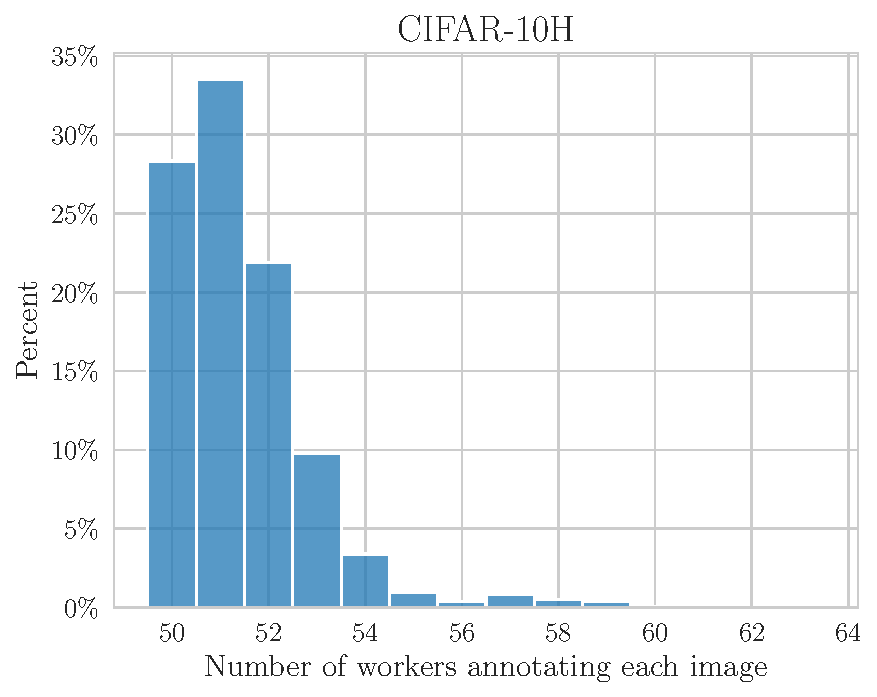
\includegraphics[trim={0 0 0 0.8cm},clip,width=0.3\textwidth]{chapters/images/distribution_feedback_effort_CIFAR-10H}\label{subfig:cifar10h_feedback_effort}} \hfill
    \subfloat[Load per worker distribution]{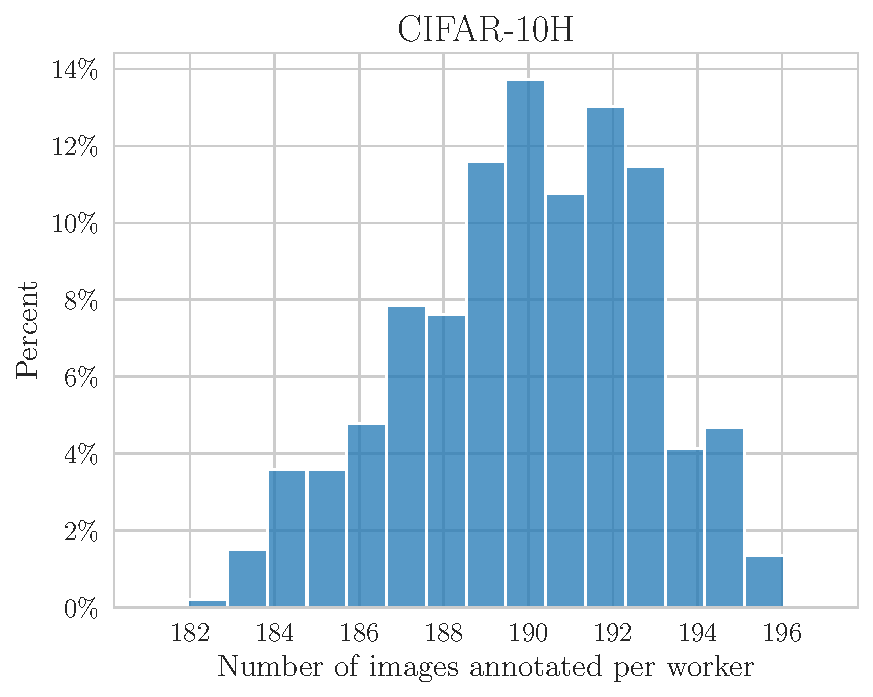
\includegraphics[trim={0 0 0 0.8cm},clip,width=0.3\textwidth]{chapters/images/distribution_workerload_CIFAR-10H}\label{subfig:cifar10h_worker_load}} \hfill
    \subfloat[Naive soft labels, entropy distribution]{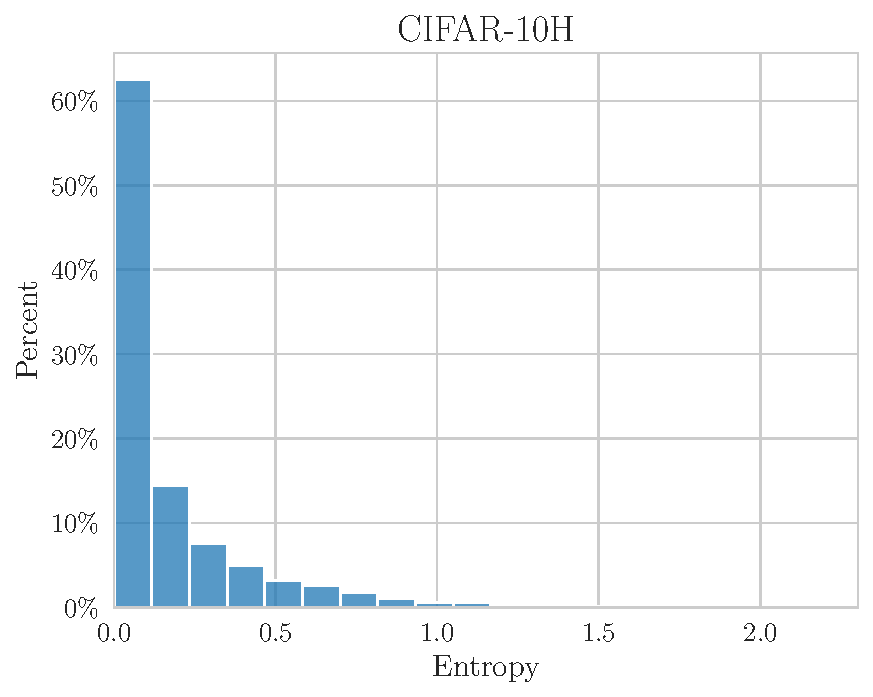
\includegraphics[trim={0 0 0 0.8cm},clip,width=0.3\textwidth]{chapters/images/distribution_entropy_CIFAR-10H}\label{subfig:cifar10h_entropy}}
    \caption{\texttt{CIFAR-10H}: dataset visualization}
    \label{fig:CIFAR-10H_dataset_visualization}
\end{figure}

From \Cref{fig:CIFAR-10H_dataset_visualization}, we can see that the creation of a validation set leads to some (small) imbalances in the load per worker and feedback effort distribution.
The entropy distribution peaks around $0$, meaning that the votes are not very ambiguous -- most tasks are easy to classify and workers agree.

\subsubsection{The \texttt{LabelMe} dataset}
\label{subsubsec:labelme}
%%%%%%%%%%%%%%%%%%%%%%%%%%%%%%%%%%%%%%%%%%%%%%%%%%%%%%%%%%%%%%%%%%%%%%%%%%%%%%%

Another real dataset in the crowdsourced image classification field that can be used is the \texttt{LabelMe} crowdsourced dataset created by \citet{rodrigues2018deep}.
This dataset consists of $n_\text{task}=1000$ training images dispatched among $K=8$ classes:
\texttt{highway}, \texttt{insidecity}, \texttt{tallbuilding}, \texttt{street}, \texttt{forest}, \texttt{coast}, \texttt{mountain} or \texttt{open country}.
The validation set has $500$ images and the test set has $1188$ images.
The whole training tasks have been labeled by $n_\texttt{worker}=59$ workers, each task having between one and three given (crowdsourced) labels.
In particular, $42$ tasks have been labeled only once, $369$ tasks have been labeled twice and $589$ received three labels.
This is a way sparser labeling setting than the \texttt{CIFAR-10H} dataset.

Also, note that the \texttt{LabelMe} dataset has classes that overlap and thus lead to intrinsic ambiguities.
This is the reason why the CoNAL strategy was introduced by \citet{chu2021learning}, see details in \Cref{subsec:conal}.
For example, the classes \texttt{highway}, \texttt{insidecity}, \texttt{street} and \texttt{tallbuilding} are overlapping for some tasks:
some cities have streets with tall buildings, leading to confusion.

\begin{figure}[thb]
    \centering
    \subfloat[Feedback effort per task]{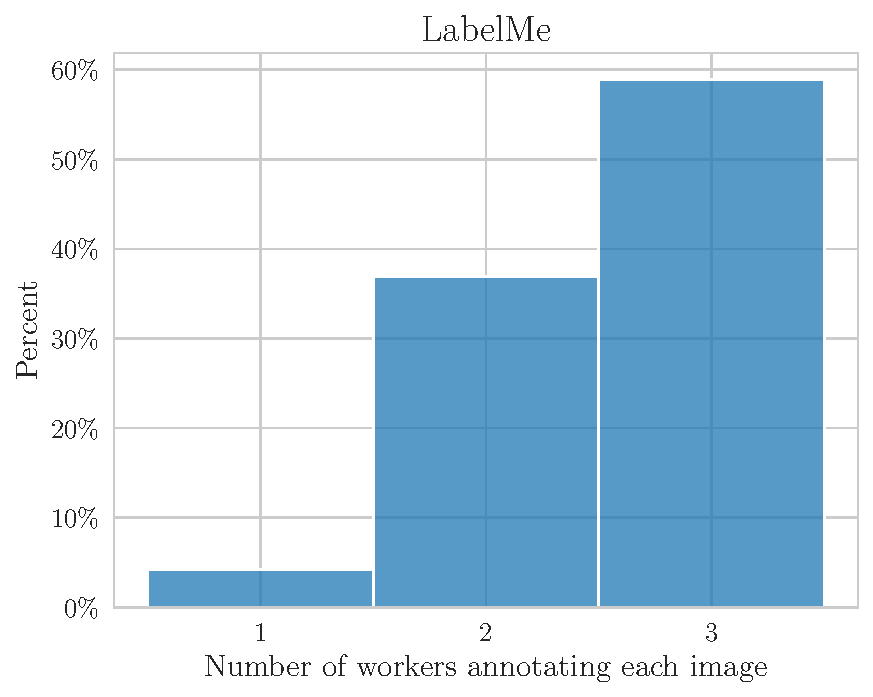
\includegraphics[trim={0 0 0 0.8cm},clip,width=0.3\textwidth]{chapters/images/distribution_feedback_effort_LabelMe}\label{subfig:labelme_feedback_effort}} \hfill
    \subfloat[Load per worker distribution]{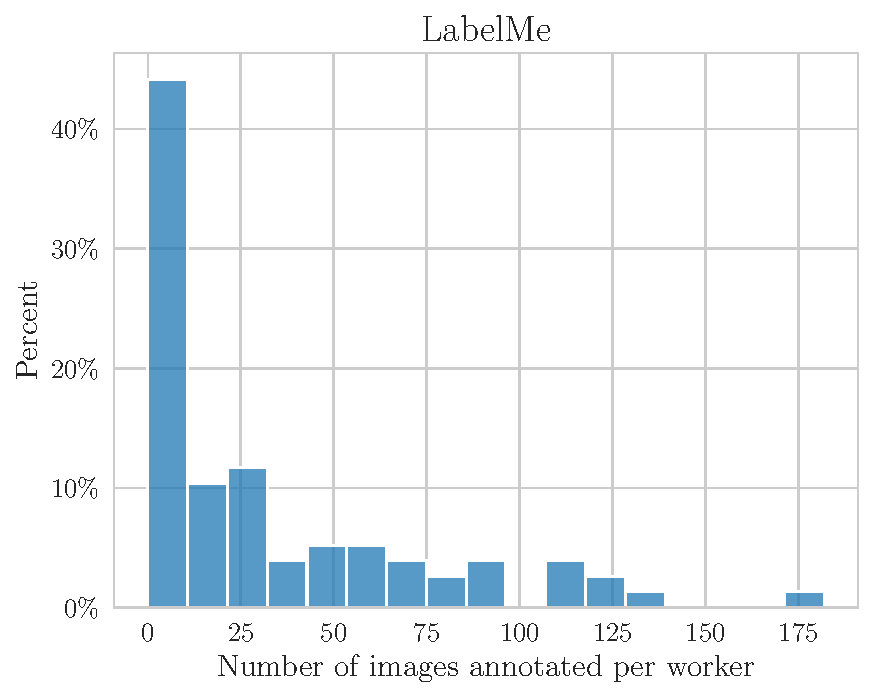
\includegraphics[trim={0 0 0 0.8cm},clip,width=0.3\textwidth]{chapters/images/distribution_workerload_LabelMe}\label{subfig:labelme_worker_load}} \hfill
    \subfloat[Naive soft labels, entropy distribution]{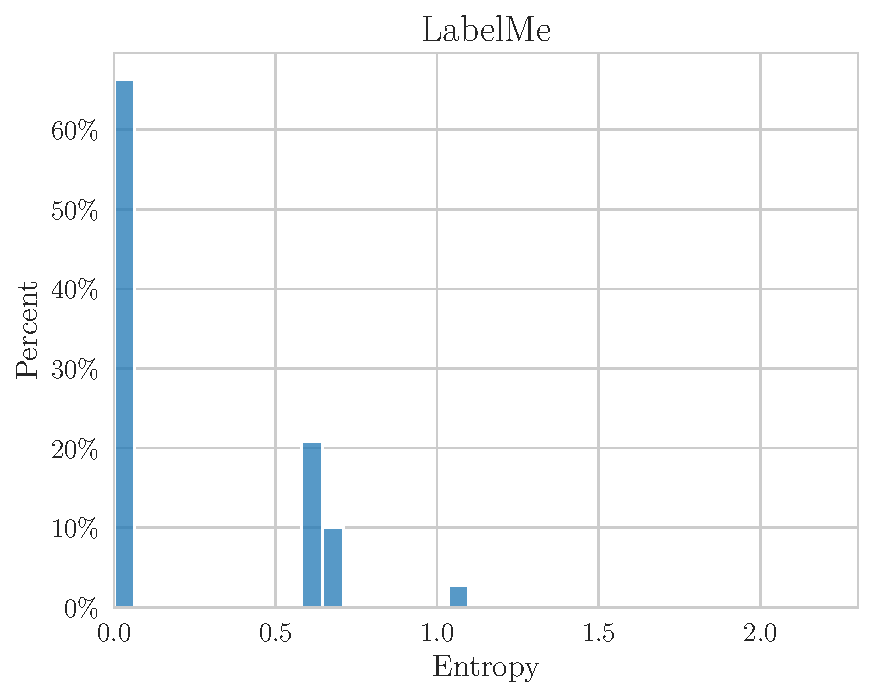
\includegraphics[trim={0 0 0 0.8cm},clip,width=0.3\textwidth]{chapters/images/distribution_entropy_LabelMe}\label{subfig:labelme_entropy}}
    \caption{\texttt{LabelMe}: dataset visualization}
    \label{fig:LabelMe_dataset_visualization}
\end{figure}

From \Cref{fig:LabelMe_dataset_visualization}, we can see that there are only up to three labels per task, leading to sparser votes per task.
Most workers answered few tasks, leading to a peak in the load per worker distribution.
There is also a vast consensus on tasks with a high peak for the entropy distribution near $0$. However, in this peak are also counted the tasks with only one label that the entropy can not separate.

%%%%%%%%%%%%%%%%%%%%%%%%%%%%%%%%%%%%%%%%%%%%%%%%%%%%%%%%%%%%%%%%%%%%%%%%%%%%%%%
\subsubsection{The \texttt{Music} dataset}
\label{subsubsec:music}
%%%%%%%%%%%%%%%%%%%%%%%%%%%%%%%%%%%%%%%%%%%%%%%%%%%%%%%%%%%%%%%%%%%%%%%%%%%%
\begin{figure}[thb]
    \centering
    \subfloat[Feedback effort per task distribution]{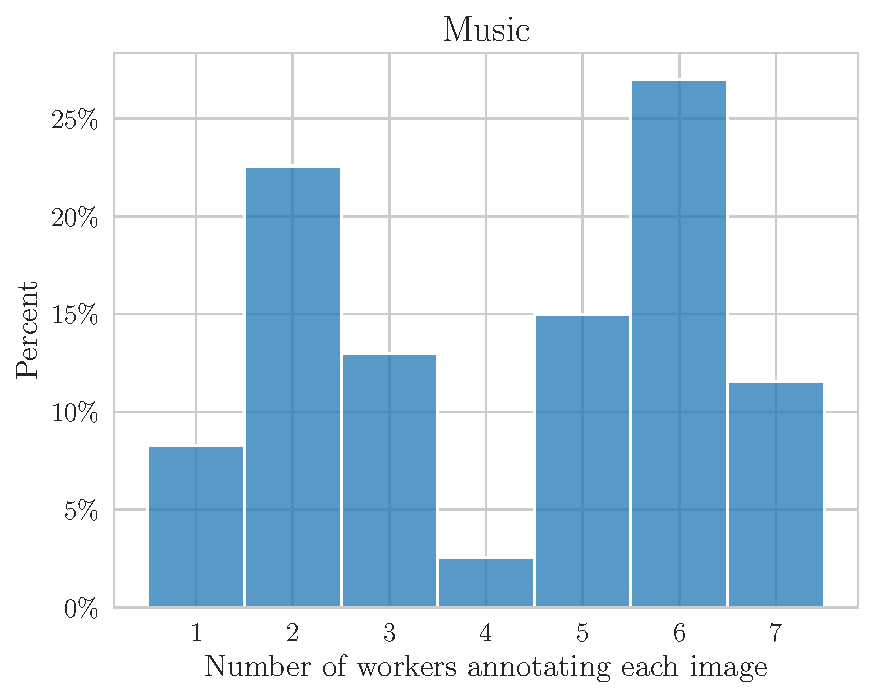
\includegraphics[trim={0 0 0 0.8cm},clip,width=0.3\textwidth]{chapters/images/distribution_feedback_effort_Music}\label{subfig:music_feedback_effort}}\hfill
    \subfloat[Load per worker distribution]{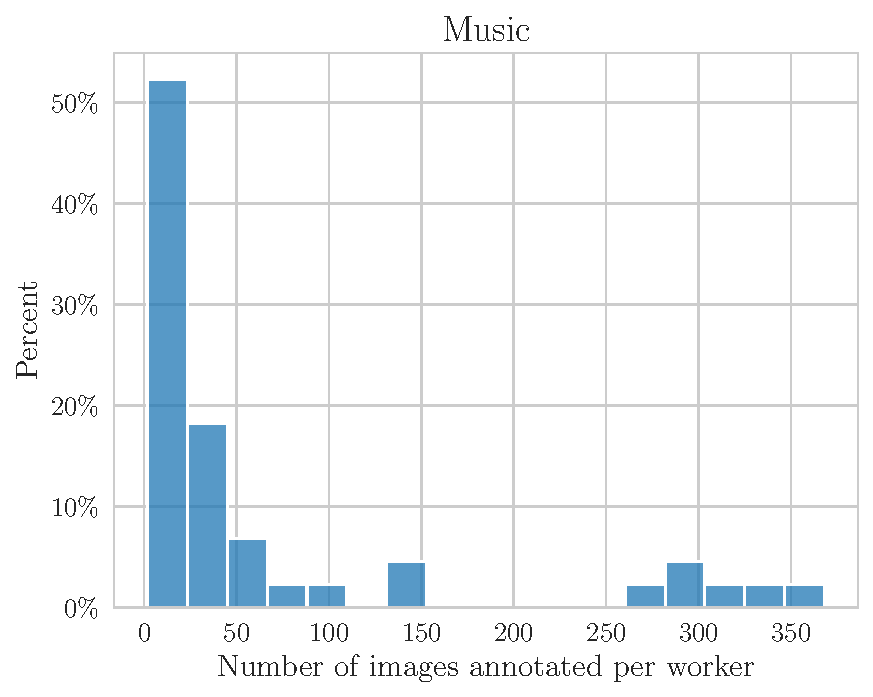
\includegraphics[trim={0 0 0 0.8cm},clip,width=0.3\textwidth]{chapters/images/distribution_workerload_Music}\label{subfig:music_worker_load}}\hfill
    \subfloat[Naive soft labels, entropy distribution]{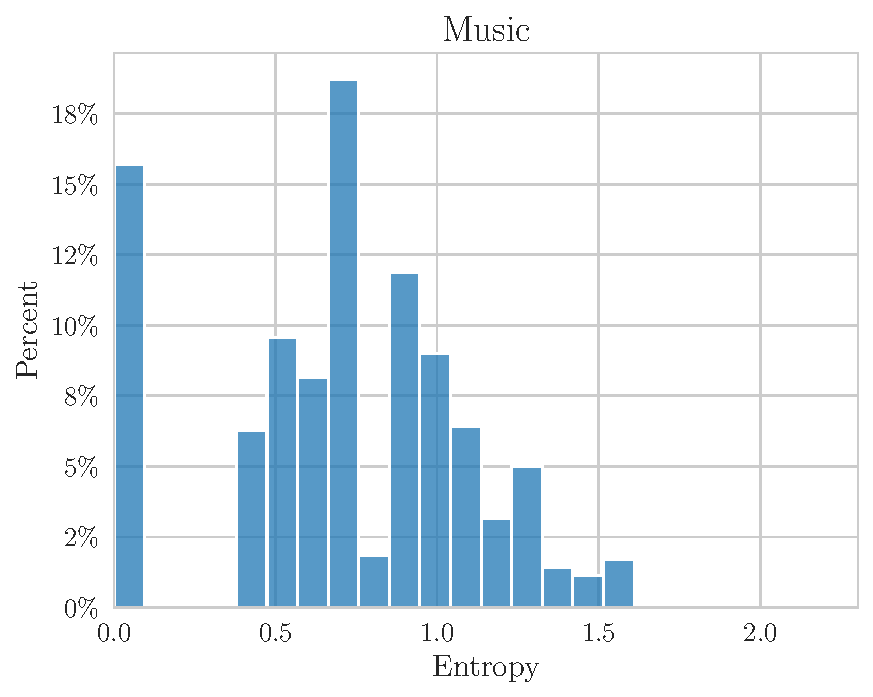
\includegraphics[trim={0 0 0 0.8cm},clip,width=0.3\textwidth]{chapters/images/distribution_entropy_Music}\label{subfig:music_entropy}}
    \caption{Music: dataset visualization}
    \label{fig:Music_dataset_visualization}
\end{figure}

\citet{rodrigues2014gaussian} released a crowdsourced dataset of audio files.
The goal of this classification task was to decide the genre of $ 30$-second musical excerpts. Number of tasks is $n_{\texttt{task}}=700$.
The $n_{\texttt{worker}}=44$ workers had $K=10$ possible labels: \texttt{blues}, \texttt{classical}, \texttt{country}, \texttt{disco}, \texttt{hiphop}, \texttt{jazz}, \texttt{metal}, \texttt{pop} and \texttt{reggae}.
Each audio file was labeled by between $1$ and $7$ workers.
To test the results, a dataset of $299$ labeled clips is used (originally $300$, but one file is known to be corrupted).
Instead of working with the original audio files, we have used Mel spectrograms, openly available\footnote{ \scriptsize \url{https://www.kaggle.com/datasets/andradaolteanu/gtzan-dataset-music-genre-classification?datasetId=568973}}, to rely on standard neural networks architecture for image classification.

From \Cref{fig:Music_dataset_visualization} we observe that each task received up to $7$ labels. Around $7.5\%$ of those tasks were annotated by a single worker. Hence the entropy can not be used to detect the ambiguity for them.
Most workers labeled few tasks, and some outliers labeled more than $300$ music recordings.

\subsection{List of publications}

This thesis is supported by the following publications:
\begin{itemize}
    \item Lefort, T., Charlier, B., Joly, A., \& Salmon, J. (2022). Crowdsourcing label noise simulation on image classification tasks. 53èmes Journées de Statistique de la SFDS 2022.
    \item Moreau, T., Massias, M., Gramfort, A., Ablin, P., Bannier, P. A., Charlier, B., \dots \& Vaiter, S. (2022). Benchopt: Reproducible, efficient and collaborative optimization benchmarks. Advances in Neural Information Processing Systems, 35, 25404-25421.
    \item Lefort, T., Charlier, B., Joly, A., \& Salmon, J. (2023) Weighting areas under the margin in crowdsourced datasets. 54èmes Journées de Statistique de la SFDS 2023.
    \item Lefort, T., Charlier, B., Joly, A., \& Salmon, J. (2024). Peerannot: classification for crowdsourced image datasets with Python. Computo (SFDS)
    \item Lefort, T., Charlier, B., Joly, A., \& Salmon, J. (2024). Improve learning combining crowdsourced labels by weighting Areas Under the Margin. TMLR.
    \item Lefort, T., Affouard, A., Charlier, B., Salmon, J., Bonnet, P. \& Joly, A. (2024). Cooperative learning of Pl@ntNet's Artificial Intelligence algorithm using label aggregation. 55èmes Journées de Statistique de la SFDS 2024
    \item Article CAP
    \item Article MEE
\end{itemize}

